\chapter{Machine Learning \ac{PSD}}
\label{chapter:ML-PSD}
This chapter will outline the main work of this thesis: different machine learning algorithms will be discussed in order to understand the effective power of such implementations for \ac{PSD} tasks in the context of LEGEND-200 signal discrimination from the background.

Firstly a \ac{VAE} model is considered: this is used with two purposes that are a classifiaction task and a denoising algorithm. Secondly a specific depp learning architecture called \ac{DTC} \cite{DTC} is investigated in order to obtain fully unsupervised clustering of waveforms and thirdly another fully-unsupervised tecnique based on humans cerebral cortex. i.e. a \ac{SOM} is used. 

\section{Data cleaning}
\label{sec:data-cleaning}
Raw charge waveforms\footnote{For \textit{raw} we mean waveforms already processed with LEGEND dedicated software, but still not selected in terms of energy, \ac{PSD} parameters or other features, as introduced at the end of Sec. \ref{subsubsec:data-structureL200}.} are not suitable for any machine learningg algorithm implementation as they are very different between one another under multiple aspects. In order to cope with this problem, a series of selection and cleaning procedures have been applied to them obtaining, at the end of said process, current waveforms in the energy range of interest.

The first data processing step that has been applied to raw waveforms is an energy-based cut around the region of interest, specifically encircling the \ac{DEP} of ${}^{208}$Tl and the \ac{FEP} of ${}^{212}$Bi. Hence, only data between 1550 keV and 1650 keV from the whole considered dataset have been saved, discarding all the other. This is a choice based on the work purposes, for which we want to neglect possibile energy-related effects on the signals and rely only on their shape evolution in time. Recalling Fig. \ref{fig:TlBi-spectrum} the energy cut is depicted in Fig. \ref{fig:cut_region} for run \textit{r000} of period \textit{p03}. Moreover data have been filtered with boolean masks provided together with raw data; said filters are needed to discard useless events. Particularly the filters that have been considered are listed in Tab. \ref{tab:quality_cuts}.

\newpage
\begin{figure}[H]
    \centering
    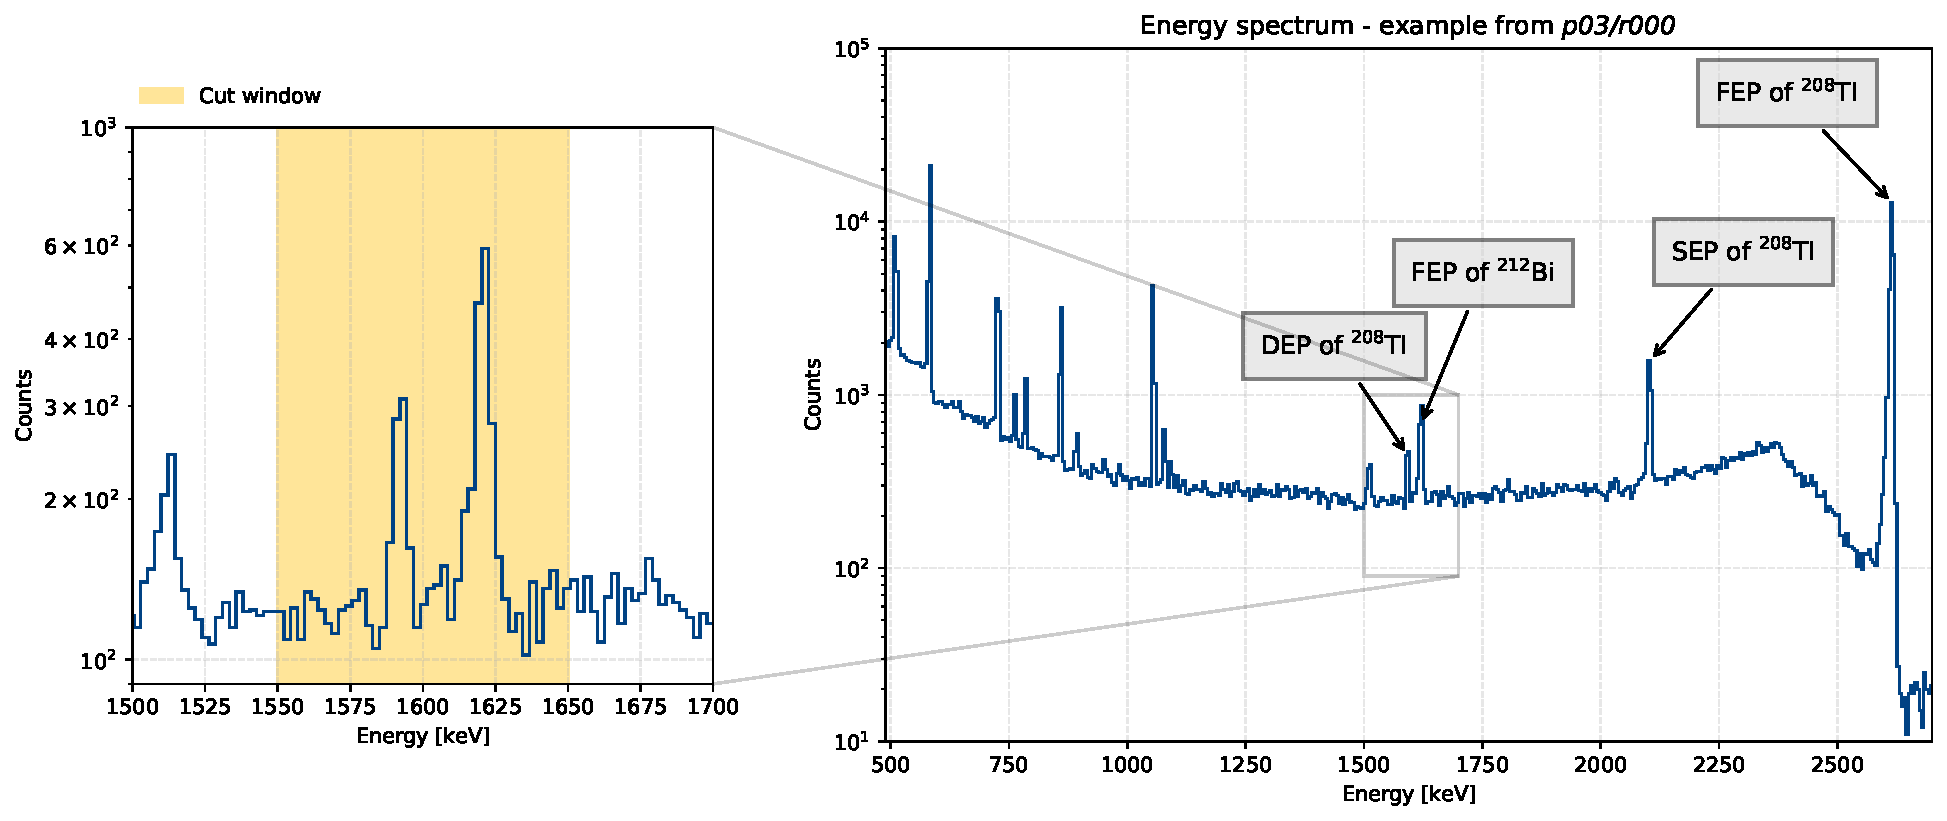
\includegraphics[width=\textwidth]{plots/energy_spectrum-cut_window.pdf}
    \caption{Example of the energy spectrum recorded in the calibration from \textit{p03/r000}. The energy region of the cut is highlighted.}
    \label{fig:cut_region}
\end{figure}

\begin{table}[H]
    \small
    \centering
    \renewcommand{\arraystretch}{1.1} % Migliora la spaziatura verticale delle righe
    \begin{tabular}{@{} l p{10cm} @{}}
        \toprule
        \textbf{Quality Cut} & \textbf{Filtered events} \\
        \midrule
        discharge & discharges events \\
        saturated & saturated waveforms (typically from muons) events \\
        baseline pile-up & events caused by high-rate overlapping in the baseline \\
        tail pile-up & events caused by high-rate overlapping in the tail \\
        valid baseline & events with noise or discontinuities in the baseline \\
        valid tail & events with noise or discontinuities in the tail \\
        valid positive leading edge & events with noise bursts in the rising edge of the waveform \\
        valid CUSP minimum energy & events dominated by electronic noise at low energies \\
        valid drift time & events with a very high drift time \\
        \bottomrule
    \end{tabular}
    \caption{Summary of Quality Cuts and discarded events considered in the data cleaning process.}
    \label{tab:quality_cuts}
\end{table}

% \begin{wrapfigure}{r}{0.6\textwidth}
%     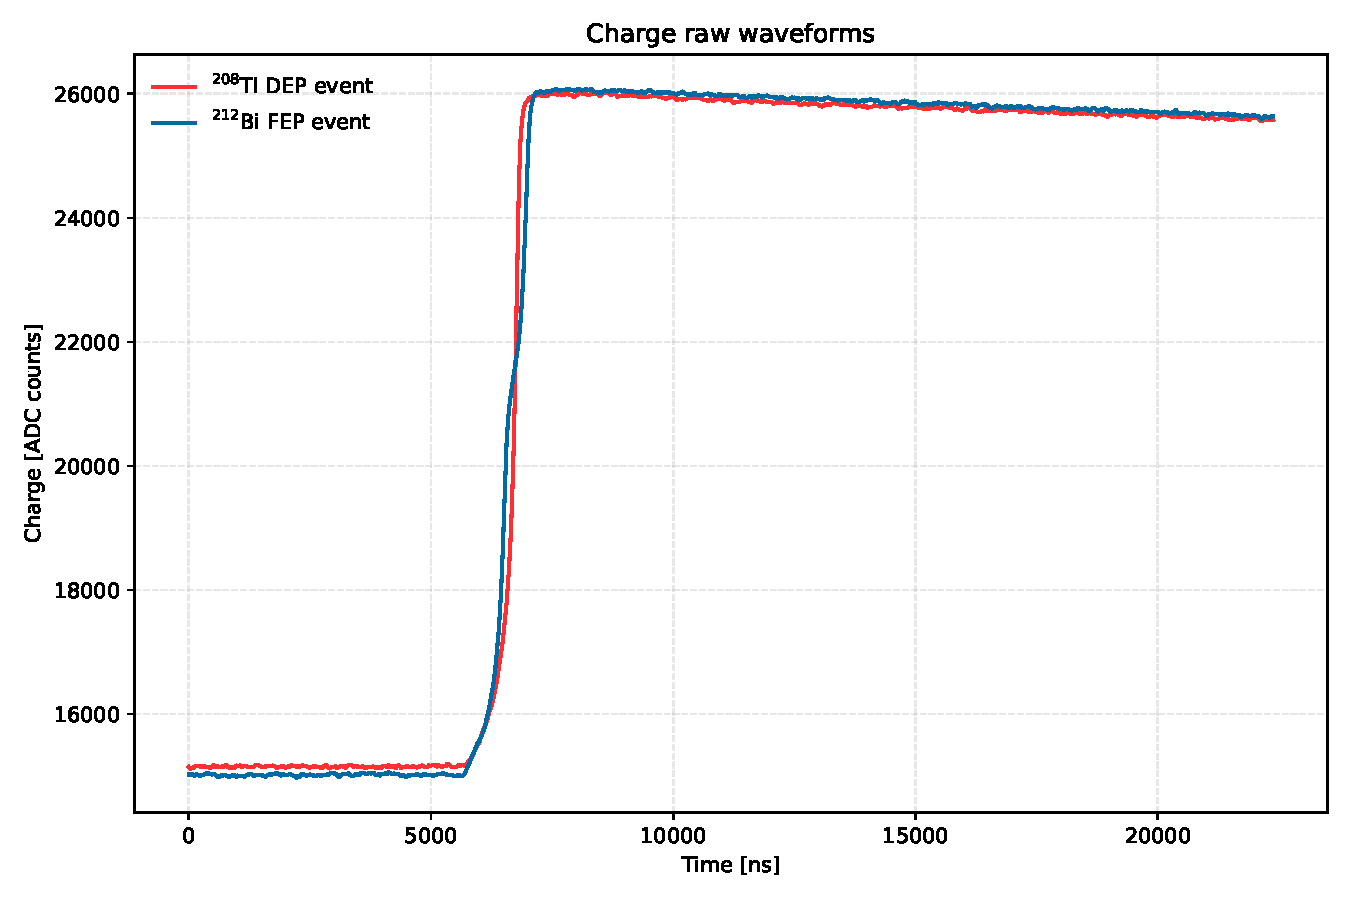
\includegraphics[width=\linewidth]{plots/wfCleaning/raw_wf.pdf}
%     \caption{Raw charge waveforms.}
%     \label{fig:raw-wf}
% \end{wrapfigure}
As soon as the energy cut and the event cut are performed, raw waveforms, as the ones in Fig. \ref{fig:a-raw} need to pass through a series of processes in order to obtain suitable inputs algorithms to be implemented. 
Firstly the mean value of the baseline is computed from the first 300 points of the raw charge waveform expressed in ADC counts and it is subtracted from all of the other points. Subsequently the baseline-subtracted charge waveform is normalised in order to have all of the waveforms with values between 0 and 1. After that, current waveforms are obtained from charge ones via time derivation using $dt = 16$~ns that arises from the sampling rate of 62.5 MHz. Current waveforms are then filtered using a Butterworth filter designed to remove high frequency parts of the signal mainly affecting the baseline part, then they are aligned with respect to the first peak of the current signal and trimmed around the alignement point with 100 samples before it and 100 after it. 
% Laslty current waveforms are normalised to their maximum: this is done because what we really want to achieve is a waveform separation purely based on their pulse shape in time; therefore every piece of information that can trace back amplitude differences or energy details needs to be removed from the algorithm input.
Once all of these steps are completed, what we obtain is a suitable input for the deep learning mdoels that are to be implemented as will be described in the nextsections. An example of the process is shown in Fig. \ref{fig:data-cleaning}, highlighting the two typical behaviours of \ac{SSE} waveforms (in red) and \ac{MSE} ones (in blue). %; examples of the other periods and runs can be found in the related Appendix \ref{app:waveforms}.

\begin{figure}[H]
    \centering
    % --- Prima figura (a) --- [ex wrapfigure]
    \begin{subfigure}[H]{0.49\textwidth}
        \centering
        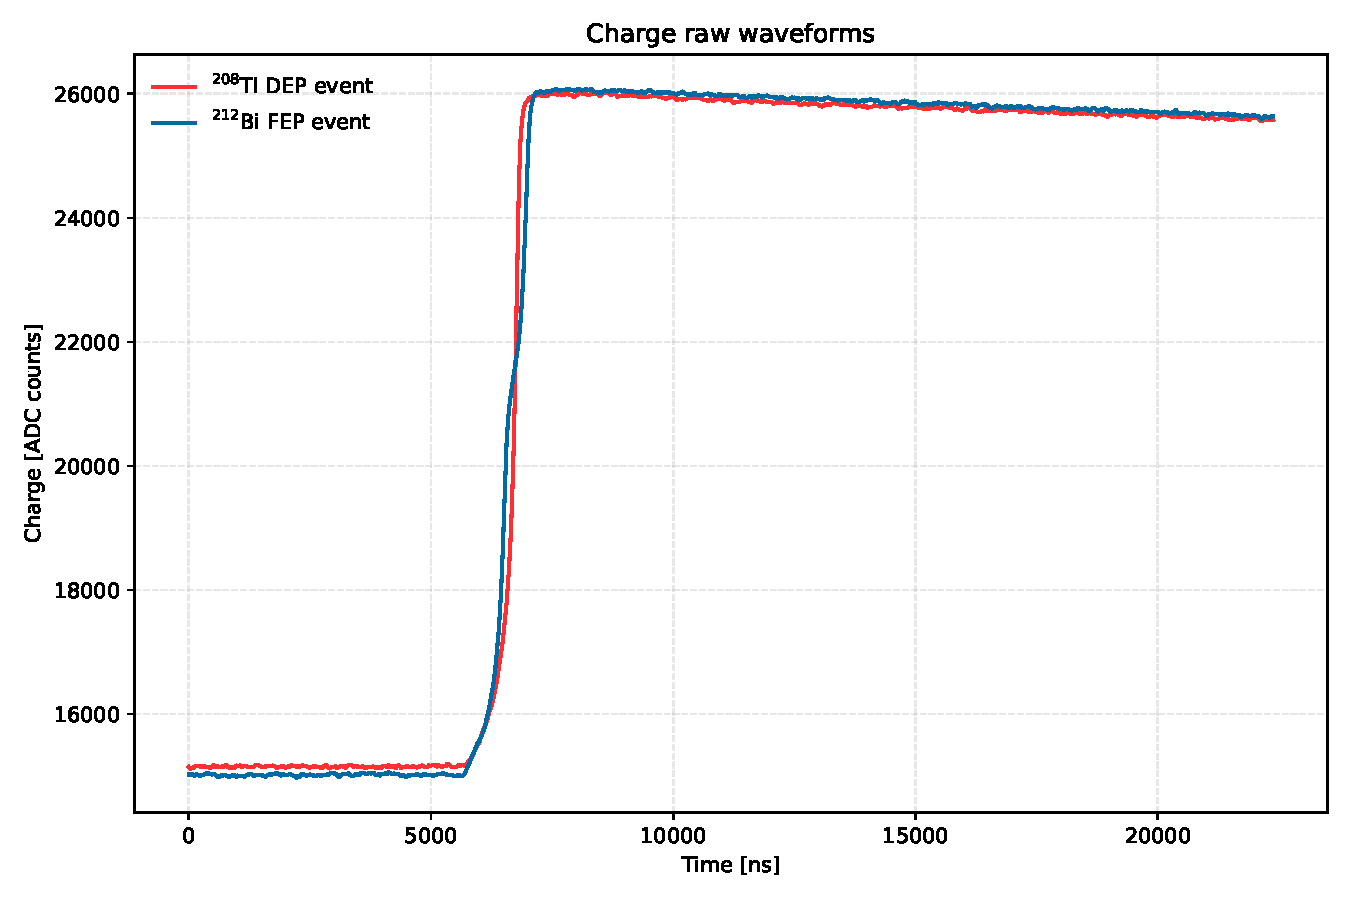
\includegraphics[width=\textwidth]{plots/wfCleaning/raw_wf.pdf}
        \caption{Raw charge waveforms.}
        \label{fig:a-raw}
    \end{subfigure}
    \hfill
    % --- Seconda figura (b) --- [ex a]
    \begin{subfigure}[H]{0.49\textwidth}
        \centering
        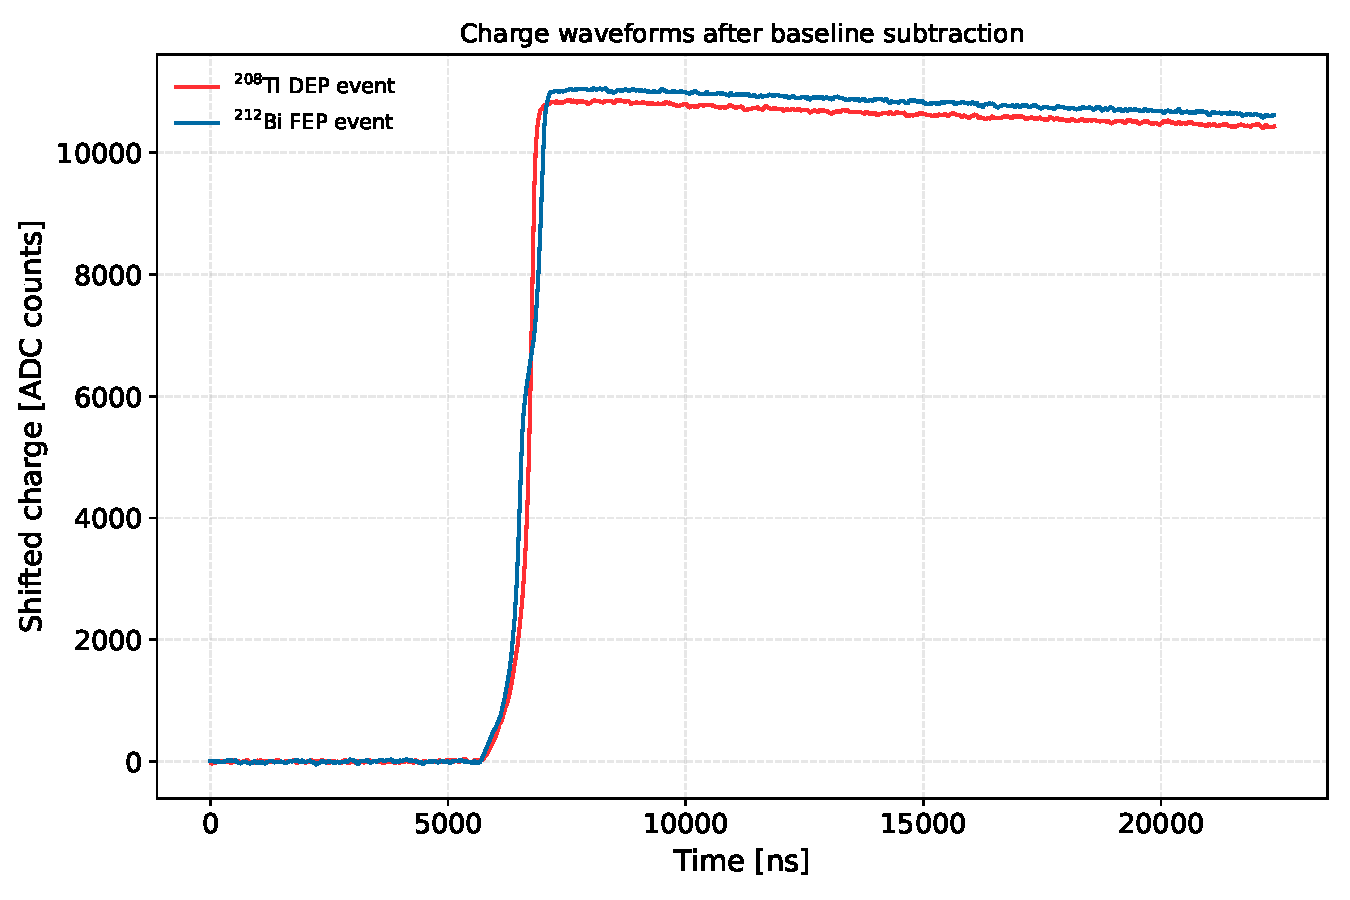
\includegraphics[width=\textwidth]{plots/wfCleaning/baseline_subtracted_wf.pdf}
        \caption{Charge waveforms after baseline subtraction.}
        \label{fig:b-baseline}
    \end{subfigure}
    
    \vspace{0.5cm} % Spazio verticale tra la prima e la seconda riga
    
    % --- Terza figura (c) --- [ex b]
    \begin{subfigure}[H]{0.49\textwidth}
        \centering
        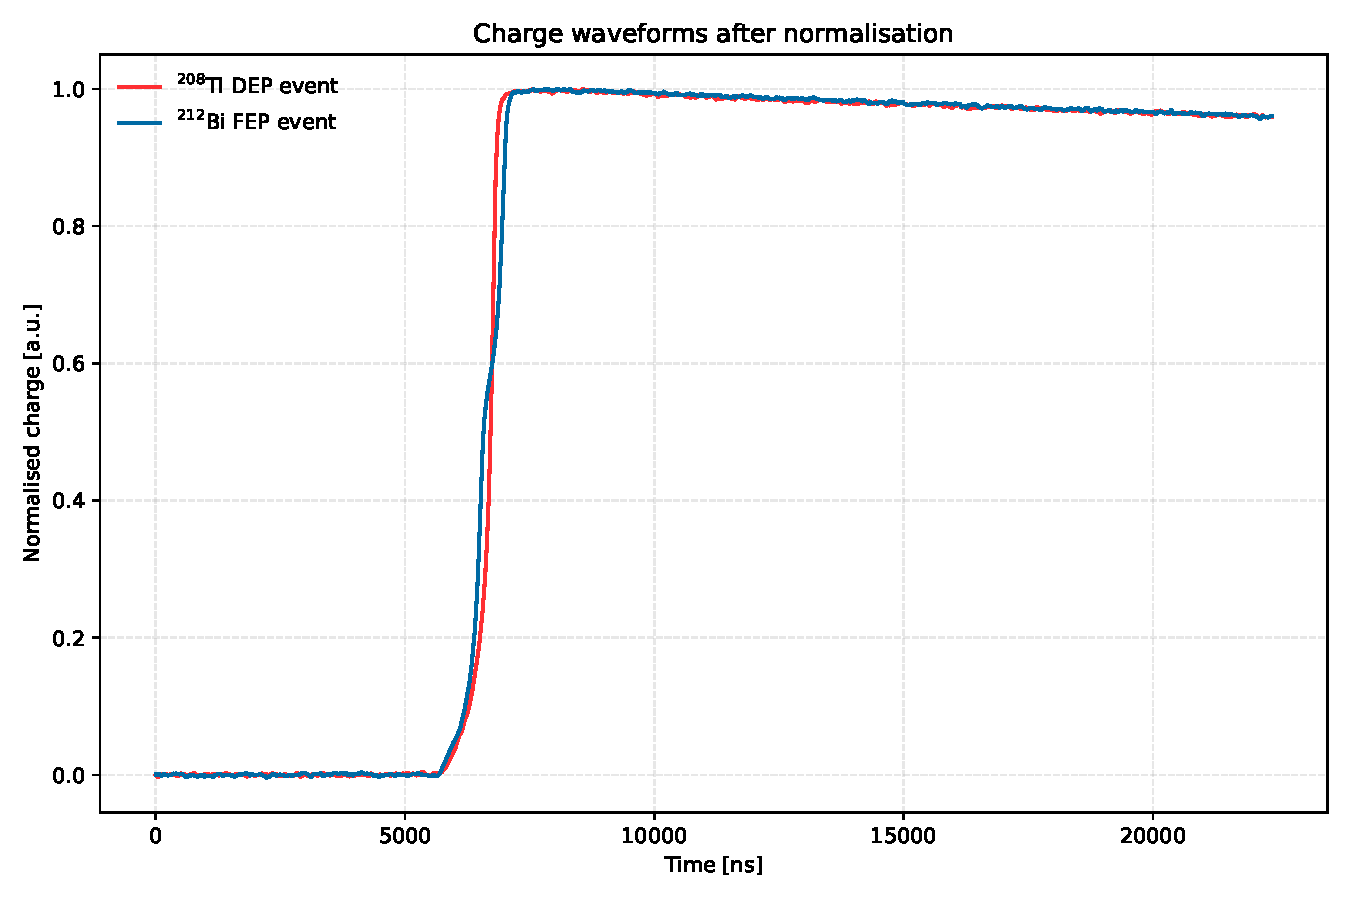
\includegraphics[width=\textwidth]{plots/wfCleaning/normalised_wf.pdf}
        \caption{Charge waveforms after normalisation.}
        \label{fig:c-normalised}
    \end{subfigure}
    \hfill
    % --- Quarta figura (d) --- [ex c]
    \begin{subfigure}[H]{0.49\textwidth}
        \centering
        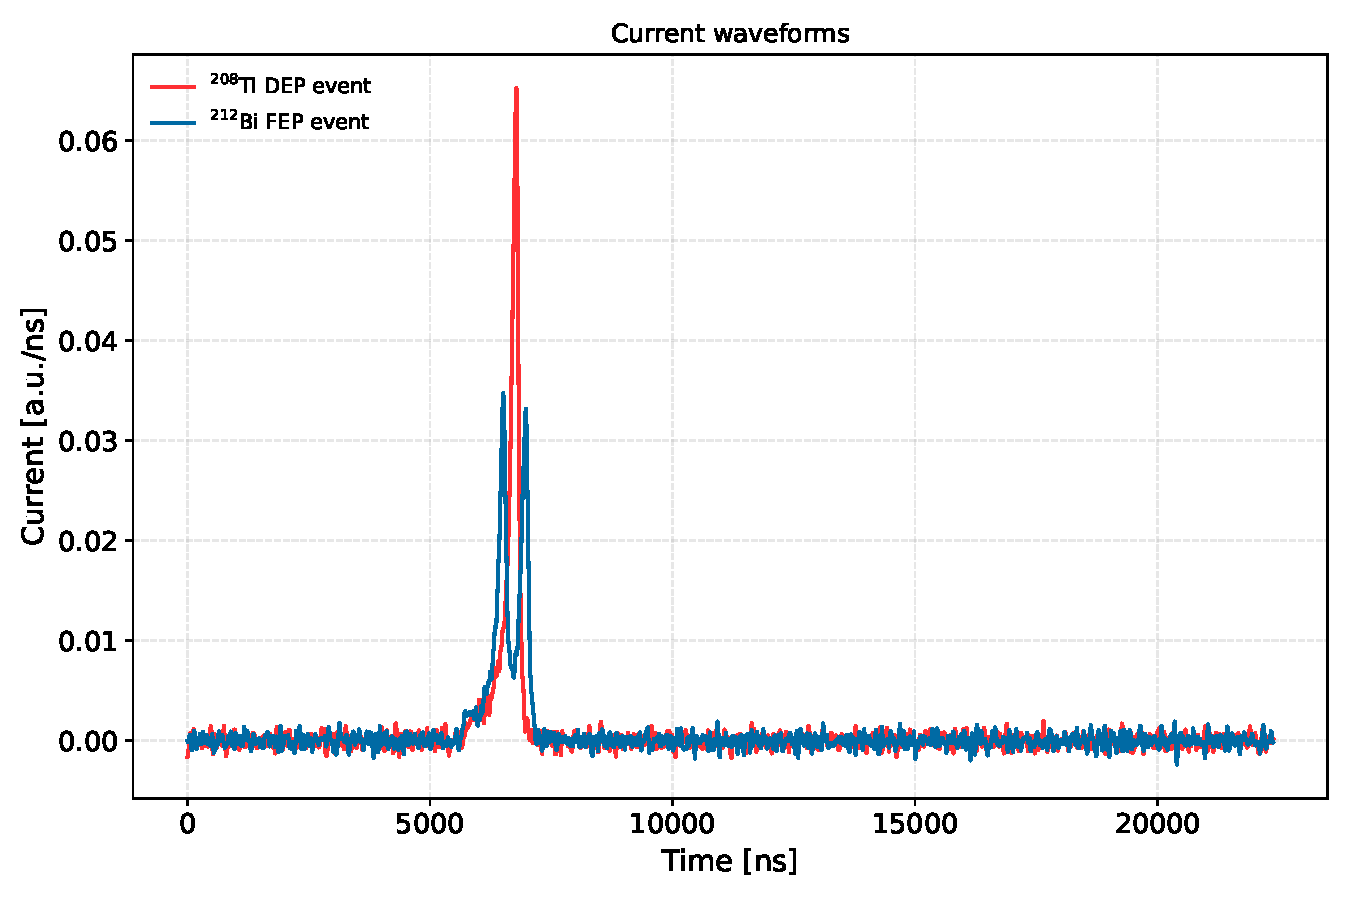
\includegraphics[width=\textwidth]{plots/wfCleaning/current_wf.pdf}
        \caption{Current waveforms obtained with time derivative.}
        \label{fig:d-current}
    \end{subfigure}

    \vspace{0.5cm} % Spazio verticale tra la seconda e la terza riga

    % --- Quinta figura (e) --- [ex d]
    \begin{subfigure}[H]{0.49\textwidth}
        \centering
        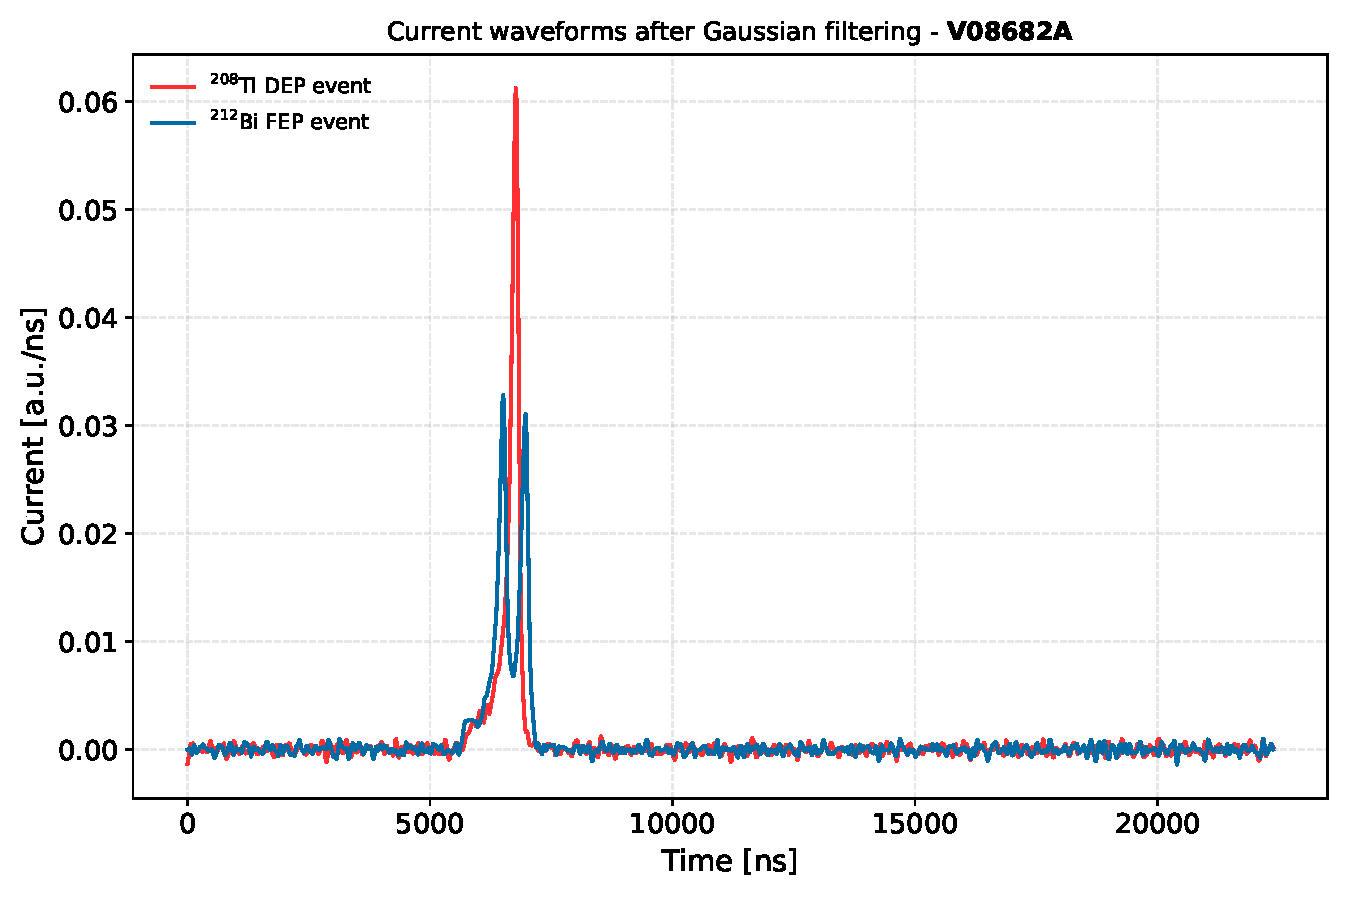
\includegraphics[width=\textwidth]{plots/wfCleaning/current_filtered_wf.pdf}
        \caption{Current waveforms after Butterworth filtering.}
        \label{fig:e-filtered}
    \end{subfigure}
    \hfill
    % --- Sesta figura (f) --- [ex e]
    \begin{subfigure}[H]{0.49\textwidth}
        \centering
        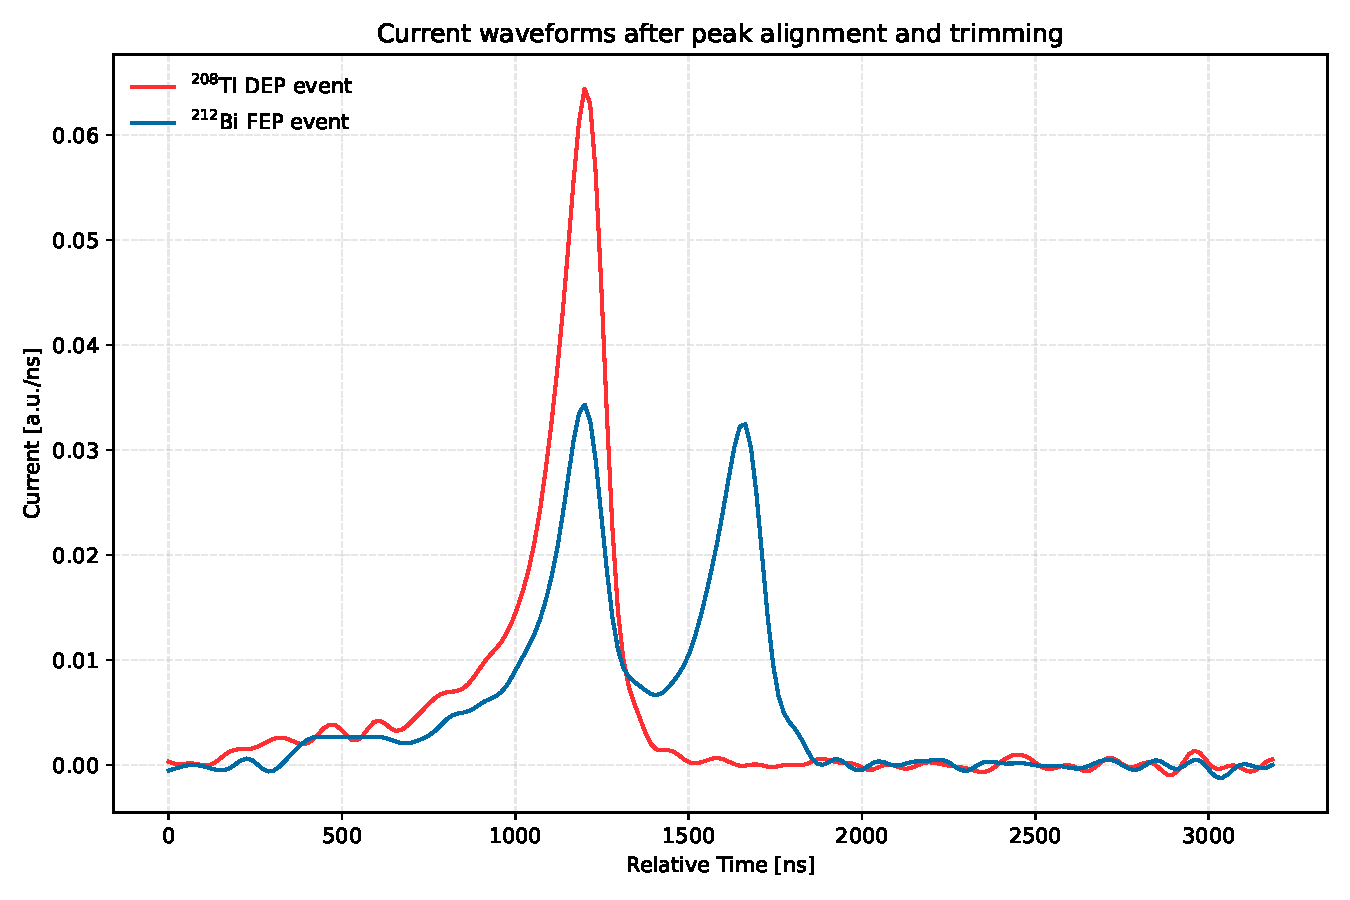
\includegraphics[width=\textwidth]{plots/wfCleaning/current_aligned_filtered_wf.pdf}
        \caption{Peak-aligned and trimmed current waveforms.}
        \label{fig:f-aligned-trimmed}
    \end{subfigure}
    
    % --- Didascalia principale ---
    \caption{Illustration of the workflow of the data processing for two types of waveforms from the dataset: the blue one is a typical \ac{MSE} waveform with a non-trivial structure while the red one is a ordinary \ac{SSE} waveform. A detailed description of the process is given in the text.}
    \label{fig:data-cleaning}
\end{figure}

\section{Data selection}
\label{sec:data-selection}

\ac{SSE} and \ac{MSE} selection is performed through the following procedure. First a gasussian fit, displayed in Fig. \ref{fig:dep_fep_fits}, is performed onto the \ac{DEP} of ${}^{208}$Tl and the \ac{FEP} of ${}^{212}$Bi via the function of Eq. \ref{eq:fitted-gaussian}
\begin{equation}
    \label{eq:fitted-gaussian}
    f(x) = A \cdot \frac{1}{\sqrt{2 \pi \sigma^2}} \cdot \exp\left(-\frac{(x - \mu)^2}{2\sigma^2}\right) + B
\end{equation}
where $A$ is the total number of events under the peak, i.e. the peak area obtained by integrating the background-subtracted Gaussian componente, $\mu$ is the mean value, $\sigma$ is the standard deviation and $B$ is the background. The results of the fit are reported in Tab. \ref{tab:gaussianfit_parameters}. 

\begin{figure}[H]
    \centering
    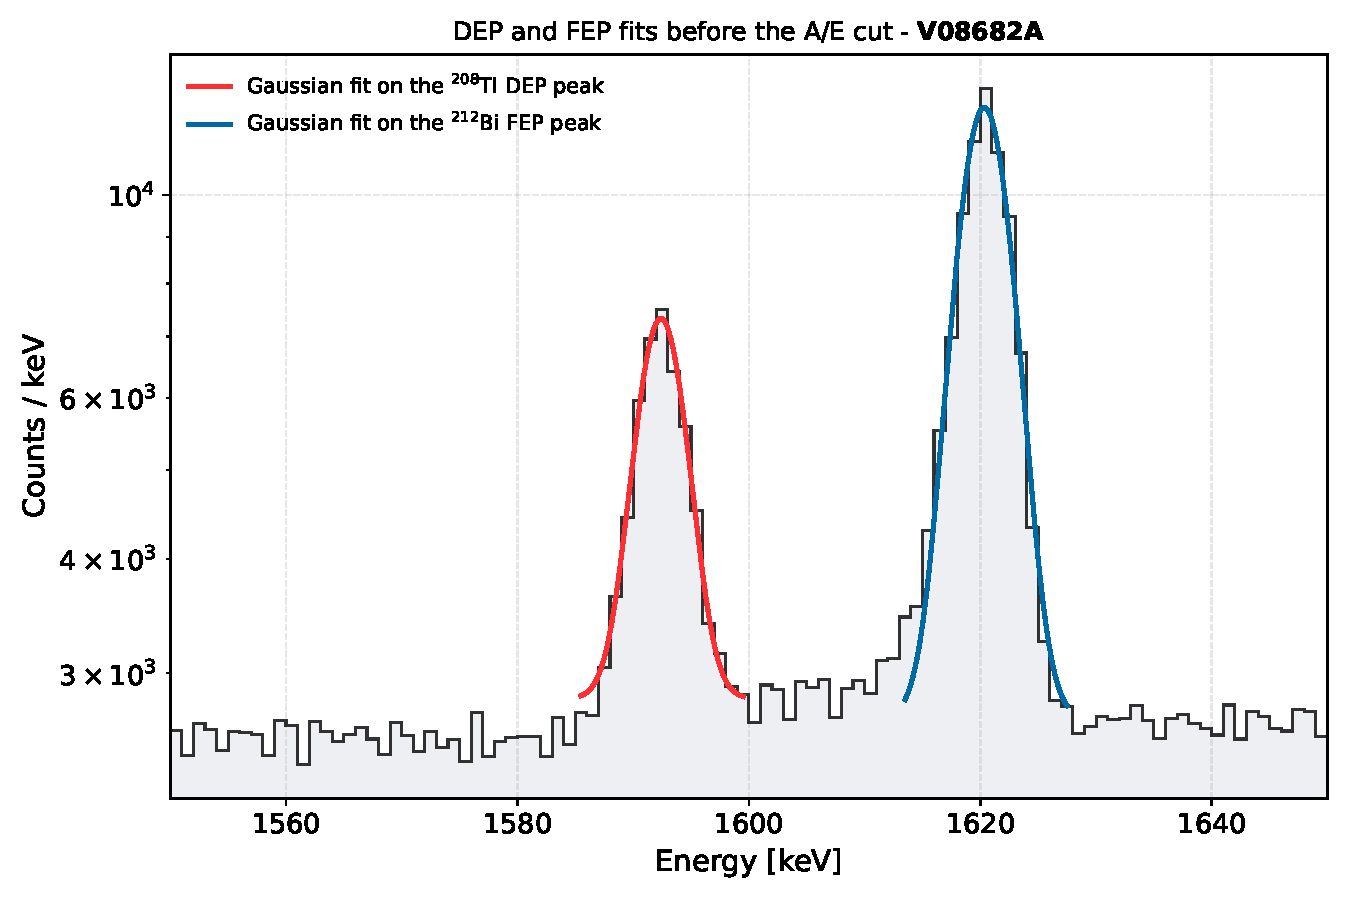
\includegraphics[width=0.8\textwidth]{plots/dep_fep_fits.pdf}
    \caption{Events selection for \ac{SSE} and \ac{MSE}. A detailed description of the procedure is given in the text.}
    \label{fig:dep_fep_fits}
\end{figure} 

\begin{table}[H]
  \centering
  \begin{tabular}{ccccc}
    \toprule
    Peak & Amplitude [counts] & $\mu$ [keV] & $\sigma$ [keV] & Background [counts/keV] \\
    \midrule
    ${}^{208}\text{Tl}$ & $(2.4 \pm 0.2) \times 10^{4}$ & $1592.40 \pm 0.06$ & $2.1 \pm 0.1$ & $(2.8 \pm 0.2) \times 10^{3}$ \\
    ${}^{212}\text{Bi}$ & $(5.7 \pm 0.7) \times 10^{4}$ & $1620.34 \pm 0.08$ & $2.3 \pm 0.2$ & $(2.7 \pm 0.6) \times 10^{3}$ \\
    \bottomrule
  \end{tabular}
  \caption{Gaussian fit parameters for the ${}^{208}\text{Tl}$ \ac{DEP} and ${}^{212}\text{Bi}$ \ac{FEP}.}
  \label{tab:gaussianfit_parameters}
\end{table}
Secondly, the selcetion needs to consider only a part of the events under the peaks. It is clear that those peaks are not purely \ac{SSE} or \ac{MSE} but rather a mixture of both since the continuum background is present in the whole energy spectrum. A cut window within a different number of sigmas would lead to different results in terms of \ac{SSE} and \ac{MSE} purity. In order to get an idea of such fractions we can consider, for different $\sigma$ cuts, the ratio between the total number of events under the peak and background part of them; these are parametrised respectively by the $A$ and $B$ paramters of Eq. \ref{eq:fitted-gaussian}.
Table~\ref{tab:purity} shows that the \ac{DEP} sample exhibits a systematically lower purity than the \ac{FEP} sample across the considered window widths. This is expected, since the \ac{FEP} peak amplitude is substantially bigger than the \ac{DEP} one while the underlying background level is comparable (see Tab.~\ref{tab:gaussianfit_parameters}), resulting in a more favourable peak-to-background ratio for the \ac{FEP} selection. This consideration is particularly relevant when we need to consider the performance of the deep learning classifier, since it is trained in a supervised mode: mislabelled events (i.e. continuum events wronlgy assigned to the \ac{SSE} or \ac{MSE} class) directly enter the loss function computation, injecting label noise that biases the training process and the resulting final performance.

\begin{table}[H]
\centering
\begin{minipage}{0.48\textwidth}
\centering
\begin{tabular}{cccc}
\toprule
$\sigma$ & peak counts & background counts & purity \\
\midrule
0.5 & 9117  & 5919  & 60.6\% \\
1.0 & 16255 & 11838 & 57.9\% \\
1.5 & 20629 & 17758 & 53.7\% \\
2.0 & 22727 & 23677 & 49.0\% \\
2.5 & 23514 & 29596 & 44.3\% \\
3.0 & 23746 & 35515 & 40.1\% \\
\bottomrule
\end{tabular}
\caption{\ac{DEP} sample}
\label{tab:purity_sse}
\end{minipage}
\hfill
\begin{minipage}{0.48\textwidth}
\centering
\begin{tabular}{cccc}
\toprule
$\sigma$ & peak counts & background counts & purity \\
\midrule
0.5 & 21873 & 6229  & 77.8\% \\
1.0 & 38996 & 12457 & 75.8\% \\
1.5 & 49489 & 18686 & 72.6\% \\
2.0 & 54523 & 24914 & 68.6\% \\
2.5 & 56412 & 31143 & 64.4\% \\
3.0 & 56968 & 37372 & 60.4\% \\
\bottomrule
\end{tabular}
\caption{\ac{FEP} sample}
\label{tab:purity_mse}
\end{minipage}
\caption{Peak counts, background counts and purity for a different number of sigmas considered in the cut window for the \ac{DEP} and \ac{FEP} samples.}
\label{tab:purity}
\end{table}



% \begin{figure}[H]
%     \centering 
%     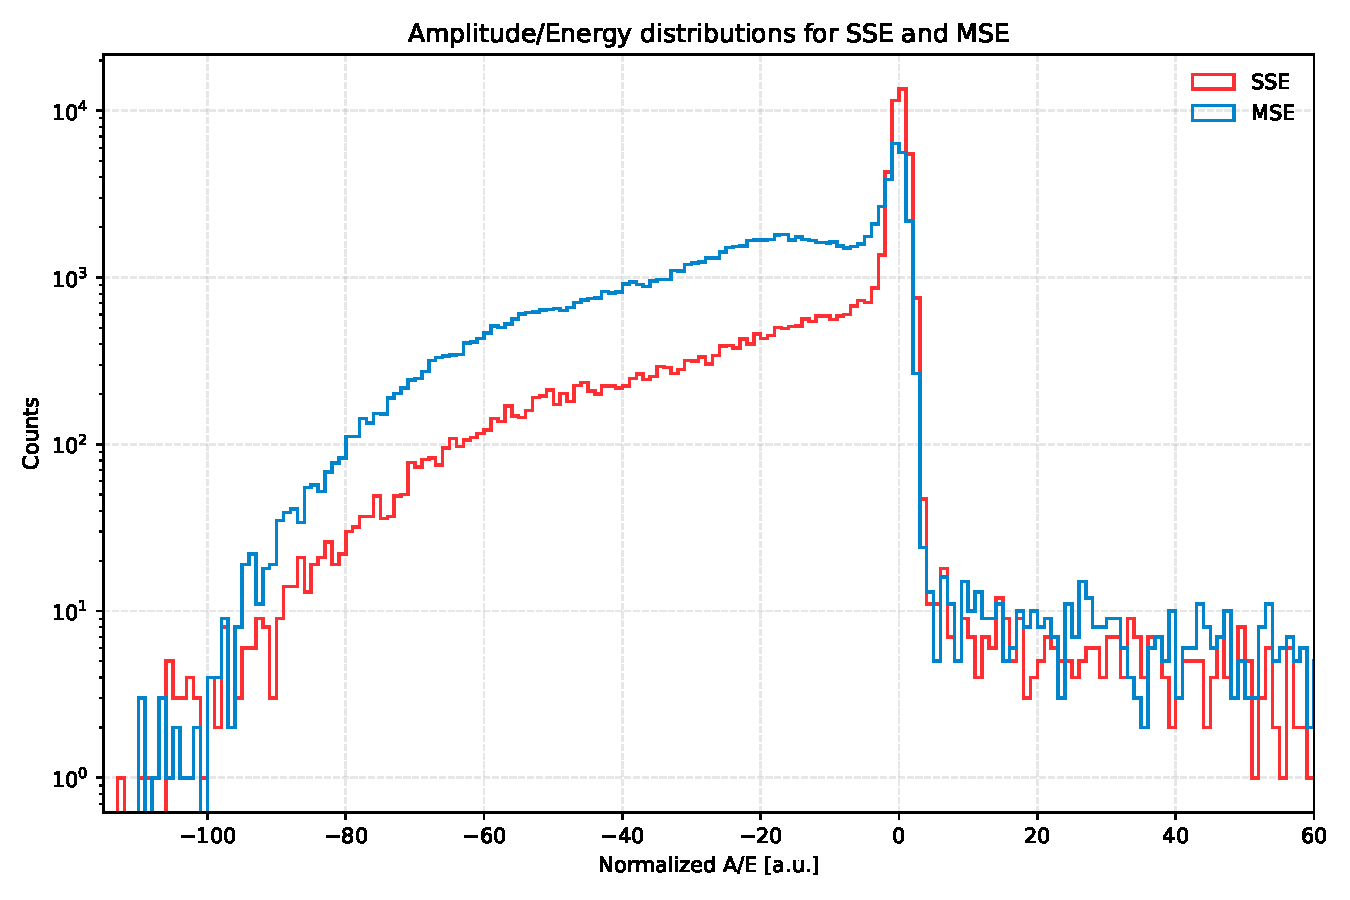
\includegraphics[width=0.7\textwidth]{plots/AoE_sse_vs_sse.pdf}
%     \caption{Distributions of the Amplitude/Energy quantity for SSE and MSE.}
%     \label{fig:AoE-sse_vs_mse}
% \end{figure}


\newpage
\section{Variational Autoencoder}
\label{sec:VAE}
A \ac{VAE} is an artificial neural network architecture itroduced by Diederik P. Kingma and Max Welling in 2013 \cite{originalVAEarticle}. These types of models connect an encoder neural network to its decoder counterpart through a probabilistic latent space, for instance Gaussian distributions. This means that the encoder maps each input point, i.e. a time series (waveform) in our case, into a distribution within the latent space, differently from the standard autoencoders where input points are mapped into a single point in the latent space. From said distributions, the decoder part reconsruct the time series. 
\subsection{Architecture}
\label{sec:vae-architeture}
\begin{comment}
QUI DEVO DIRE

-COME CREO I TENSORS --> TENSORCREATION.PY

-COME IMPLEMENTO IL VAE

    - encoder\\
    - decoder\\
    - latent space specifications\\
    - costruzione della loss\\
    - training\\ 
    - test\\
    - tutti i test del codice che faccio\\
        * test su beta
        * test su dimensioni dello spazio lentamente
        * eventuale PCA e/o TRAVERSAL
- COME IMPLEMENTO LA CLASSIFICATION\\
    - layers etc\\ 
    - loss\\
    - training \\
    - test \\
\end{comment}
The \ac{VAE} algorithm that has been implemented in the work here presented follows a simple flow which includes an encoder, a 8-dimension latent space, a reparametrisation step and a decoder. The steps, also illustrated in Fig. \ref{fig:vae-architecture}, include: 
\begin{itemize}
    \item \textbf{original waveforms}\\
    The input of the encoder are charge and current waveforms already processed as described in Sec. \ref{sec:data-cleaning}. Specifically, it can be defined whether to use as input only current or charge waveforms or both of them simoultaneously, tuning a dedicated parameter called \texttt{channels}. Therefore the input of the encoder have overall dimensions (\texttt{channels} $\times~200$)
    \item \textbf{encoder}\\
    The encoder is defined within a sequential conatiner (\texttt{class torch.nn.Sequential} \cite{torchSequential}), therefore modules are added to it in the order they are passed. Specifically the modules are:
    \begin{enumerate}
        \item a 1D convolutional layer (\texttt{Conv1d} in PyTorch) with kernel size = 5, stride = 2 and padding = 2, mapping (\texttt{channles} $\times 200$) inputs into (16 $\times~100$) objects;
        \item a Leaky ReLU activation, that is a similar to a Rectified Linear Unit function as detailed in Eq. \ref{eq:leakyReLU} where $\alpha = 0.1$
        \begin{equation}
            \label{eq:leakyReLU}
            f(x) = 
            \begin{cases} 
                x & \text{if } x > 0 \\
                \alpha \cdot x & \text{if } x \le 0 
            \end{cases}
        \end{equation}
        \item another 1D convolutional layer with kernel size = 5, stride = 2 and padding = 2, , mapping (16 $\times 100$) objects from the previous layer into ($32~\times~50$) outputs;
        \item another Leaky ReLU activation function identical to the previous one.
    \end{enumerate} 
    \item \textbf{latent space}\\
    The latent space is constructed from the output of the encoder after the following procedure:
    \begin{enumerate}
        \item firstly, the encoder output is flattened to a sequence with $32~\times~50$ points;
        \item a 1D convolutional layer (\texttt{Conv1d} in PyTorch) with kernel size = 5, stride = 2 and padding = 2, mapping (\texttt{channles} $\times 200$) inputs into (16 $\times~100$) objects;
        \item secondly, the flattened data are passed through a linear layer (\texttt{Linear} in PyTorch) which further reduce the dimensionality to 64 points;
        \item thirdly, a Leaky ReLU activation with $\alpha=0.1$ is applied;
        \item lastly, parameters of the latent space are obtained separately with another linear layer (\texttt{nn.Linear}) that maps the 64 activated points to a number of ($\mu$, $\sigma$) couples: said number is defined with the appropriate parameter and is the dimension of the latent space.
    \end{enumerate}
    \item \textbf{reparametrisation and decoder input}\\
    The latent space consists of $\mu$ and $\sigma$ values defining non-differentiable Gaussians distributions; however, being a gradient-based architecture, the \ac{VAE} requires differentiable functions to update the weights of the neural network via backpropagation and thus it is incompatible with the abovementioned distributions. A trick called \textit{reparametrisation trick} is employed to obtain a differentiable function starting from ($\mu$, $\sigma$) values. Specifically a new variable \textit{z} is defined as reported in Eq. \ref{eq:reparametrisation-trick} where $\varepsilon$ is a parameter casually sampled from a normal distribution (mean 0 and variance 1).
    \begin{equation}
        \label{eq:reparametrisation-trick}
        z = \mu + \varepsilon \cdot \sigma
    \end{equation}
    The appropriate input for the decoder network is computed from the $z$ values (one for each dimension in the latent space), by applying a linear layer returning 64 points followed by the usual Leaky ReLU activation and then another linear layer returning 1600 points activated again with the Leaky ReLU. The obtained object has dimensionality ($50~\times~32$) just as the output of the encoder and is a suitable input for the decoder.
    \item \textbf{decoder}\\
    The decoder perfectly mirrors the encoder: 
    \begin{enumerate}
        \item the ($50~\times~32$) input is upsampled in linear mode (i.e. using a linear regression) in order to obtain a ($32~\times~100$) object ;
        \item a 1D convolutional layer with kernel size = 5, stride = 1 and padding = 2 is exploited to extract patterns and smooth out the upsampling output returning a ($16~\times~100$) object;
        \item another linear upsampling modifies the dimensionality to ($16~\times~200$);
        \item the final 1D convolutional layer returns a original-waveform like output (\texttt{channels} $\times~200$)
    \end{enumerate}  
    \item \textbf{reconstructed waveforms}: the output of the decoder, i.e. the output of the whole \ac{VAE} is the recontruction of the input, therefore what we obtain are current, charge or both waveforms reconstructed using information extracted from the latent space. 
\end{itemize}  
\begin{figure}[H]
    \centering
    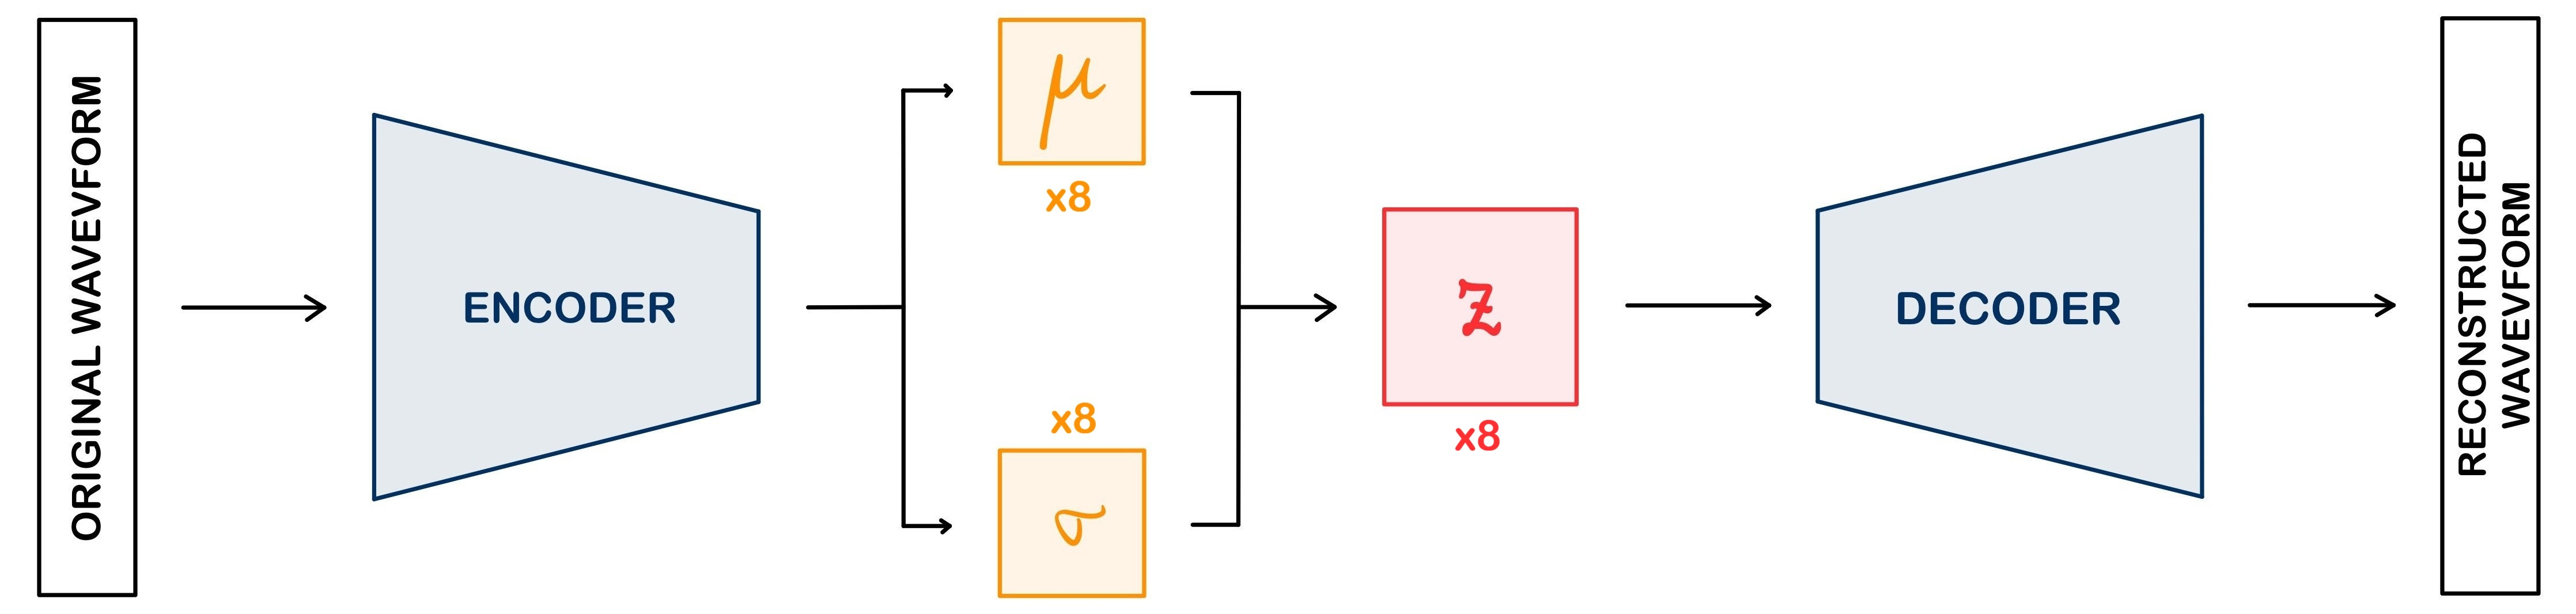
\includegraphics[width=\textwidth]{figures/schemaVAE.jpg}
    \caption{Schematic representation of the VAE architecture. The encoder network maps the input waveform to a latent space characterized by a mean and variance, from which a latent vector is sampled. The decoder reconstructs the waveform from this latent representation. The loss function combines reconstruction loss and KL divergence, weighted by the hyperparameter.}
    \label{fig:vae-architecture}
\end{figure}



\subsection{Training and testing}
\label{subsec:VAE-training}
The loss function that have been used is an \ac{ELBO}, i.e. the characteristic loss implemented in \ac{VAE} models, with some adjustments created for our specific work. The general formula is written in Eq. \ref{eq:ELBO} where it is visible that two terms enters in the loss computation: a reconstruction term and a regularisation one.
\begin{equation}
    \label{eq:ELBO}
    L = L_{\text{rec}} + \beta \cdot L_{\text{reg}}
\end{equation}

In the context of a \ac{VAE}, using a standard Mean Squared Error for the reconstruction loss would force the model to reproduce both the physically significant features of the waveform and the background stochastic noise, such as the random fluctuations preceding and following the main peaks. To overcome this limitation, the reconstruction term in the \ac{ELBO} function is modeled as the (\ac{NLL}) of a Gaussian distribution. Instead of assuming a fixed noise level, the \ac{VAE} dynamically learns a channel-specific variance, denoted as $\sigma_c^2$. This allows the model to weight the reconstruction error with respect to the expected noise level of each specific channel $c$.
Mathematically speaking, the squared error is divided by the learned variance $\sigma_c^2$, and a logarithmic penalty term ($\log \sigma_c^2$) is added. This second term is crucial to prevent a trivial solution: if the loss only consisted of the first term ($( x_{i,c,t} - \hat{x}_{i,c,t} )^2 / \sigma_c^2$), the optimization algorithm would simply predict an infinitely large noise value to drive the error to zero. The addition of the logarithmic penalty forces the model to find an optimal balance, preventing the overestimation of the underlying noise.
In this specific work, the two channels of the input tensor represent the charge and the current of the same physical signal. Since current is the time derivative of charge, these two quantities inherently possess fundamentally different scales and noise profiles. By learning a separate $\sigma_c^2$ for each channel, the \ac{NLL} acts as an automatic normalization mechanism, preventing the channel with the larger numerical magnitude or higher intrinsic variance from dominating the loss gradient. 
Finally, the individual losses of the channels must be summed, as expressed in Eq. \ref{eq:rec-loss}. From a probabilistic poin of view, this is equivalent to assuming independence of the noise between the charge and current measurements. Moreover, this sum is necessary to aggregate the array of channel-specific errors into a single scalar value, which is required by the framework to correctly perform the backpropagation algorithm.
\begin{equation}
    \label{eq:rec-loss}
    L_{\text{rec}} = \frac{1}{B} \sum_{i=1}^{B} \sum_{c=1}^{C} \left[ \frac{1}{2} \sum_{t=1}^{T} \left( \frac{\left( x_{i,c,t} - \hat{x}_{i,c,t} \right)^2}{\sigma_c^2} + \log \sigma_c^2 \right) \right]
\end{equation}

The second part of the loss expressed in Eq. \ref{eq:ELBO} concerns the organisation of the 8-dimension latent space and is based on \ac{KL} divergence. Firstly we define a \textit{prior} distribution, i.e. a standard Gaussian distribution $p(z) = \mathcal{N}(z; \mathbf{0}, \mathbf{I})$ with a zero mean vector and an identity covariance matrix. Secondly, seeing that the encoder network maps the original input waveform $x$ into a set of 8 Gaussian distributions, we can define the so-called \textit{posterior} distribution $q(z|x) = \mathcal{N}(z; \boldsymbol{\mu}_\phi(x), \text{diag}(\boldsymbol{\sigma}_\phi^2(x)))$, parameterized by the learned mean and variance vectors.
The \ac{KL} divergence is then computed to measure the statistical distance between the approximate \textit{posterior} and the \textit{prior}. This penalizes the model if the latent representations deviate significantly from a standard normal distribution. For a single latent dimension $j$, computed over a batch of size $B$, the analytical closed-form of the \ac{KL} divergence is given in Eq. \ref{eq:KL-loss}:
\begin{equation}
    \label{eq:KL-loss}
    D_{\text{KL},j} = \frac{1}{B} \sum_{i=1}^{B} \frac{1}{2} \left( \mu_{ij}^2 + \sigma_{ij}^2 - 1 - \log \sigma_{ij}^2 \right)
\end{equation}
In standard \ac{VAE} training, forcing strong regularization can lead to \textit{posterior collapse}: this occurs when the optimization algorithm drives the \ac{KL} divergence to zero by collapsing the posterior distribution to identically match the prior, effectively ignoring the input data and preventing the encoder from learning meaningful representations. 
To prevent this issue, a ``free bits'' (or \ac{KL} thresholding) strategy is implemented. Instead of forcing the divergence of every dimension to reach absolute zero, a minimum threshold $\lambda_{fb}$ is established. The total regularization loss $L_{\text{reg}}$ is computed by clamping the \ac{KL} divergence of each dimension to this lower bound before summing them, as defined in Eq. \ref{eq:KL-total} where $k$ is the number of dimensions in the latent space.
\begin{equation}
    \label{eq:KL-total}
    L_{\text{reg}} = \sum_{j=1}^{k} \max \left( \lambda_{fb}, \, D_{\text{KL},j} \right)
\end{equation}
By applying this maximum operator, the network is not forced to perfectly match the \textit{prior} distribution. If the divergence $D_{\text{KL},j}$ of a specific dimension drops below the chosen threshold $\lambda_{fb}$, the loss for that dimension remains constant at $\lambda_{fb}$. This means the encoder is allowed to retain a small amount of useful information (the \texttt{free bits}) to describe the waveform without being further penalized by the optimization process, effectively preventing the posterior collapse.

An additional tunable parameter $\beta$ balances the two contributions in the loss function: when $\beta < 1$ the reconstruction error weights more than the \ac{KL} thus the algorithm favours a truthful reconstruction, on the other hand if $\beta > 1$ the \ac{KL} becomes more important than the reconstruction. During the first part of the training a number $N_w$ of \textit{warm-up epochs} use a variable value of $\beta$ that is then settle to 1 as defined in Eq. \ref{eq:beta} where $n$ is the epoch number. This procedure is defined in order to let the algorithm learn appropriate weights for the reconstruction before trying to minimise the \ac{KL} divergence.
\begin{equation}
    \label{eq:beta}
    \beta(n) = \beta \cdot \min\left(1, \frac{n+1}{N_{\text{w}}}\right)
\end{equation}

The training and testing of the algorithm is done splitting the dataset in order to have the 90\% of the total available data for the training and validation sets and the 10\% of them for the test set.
Said 90\% is then splitted again, keeping the 90\% of it for the training set and the 10\% for the validation one. A number $N_w = 10$ of warm-up epochs have been used during the training phase of this algoritm. The number of dimensions in the latent space is $k = 8$.

The two following sections (\ref{subsec:VAE-features_extraction} and \ref{subsec:VAE-denoising}) will discuss two possible outcomes of the \ac{VAE} model, a feature extractor for a classification task and a denoising algorithm for current waveforms. However an initial verification of the robustness of its ability in the pure reconstruction task allows us to ensure the fact that if the reconstruction follows the waveform shape, the latent space is representative of the input as a consequence. Fig. \ref{fig:esempio-ricostruzione} and \ref{fig:esempio-losses} displays the reconstruction flow throught 100 epochs using $\beta=1$ and considering events within $3\sigma$ of the \ac{DEP} and \ac{FEP} as depicted in Fig. \ref{fig:sse_mse_cut}.

\begin{figure}[H]
    \centering
    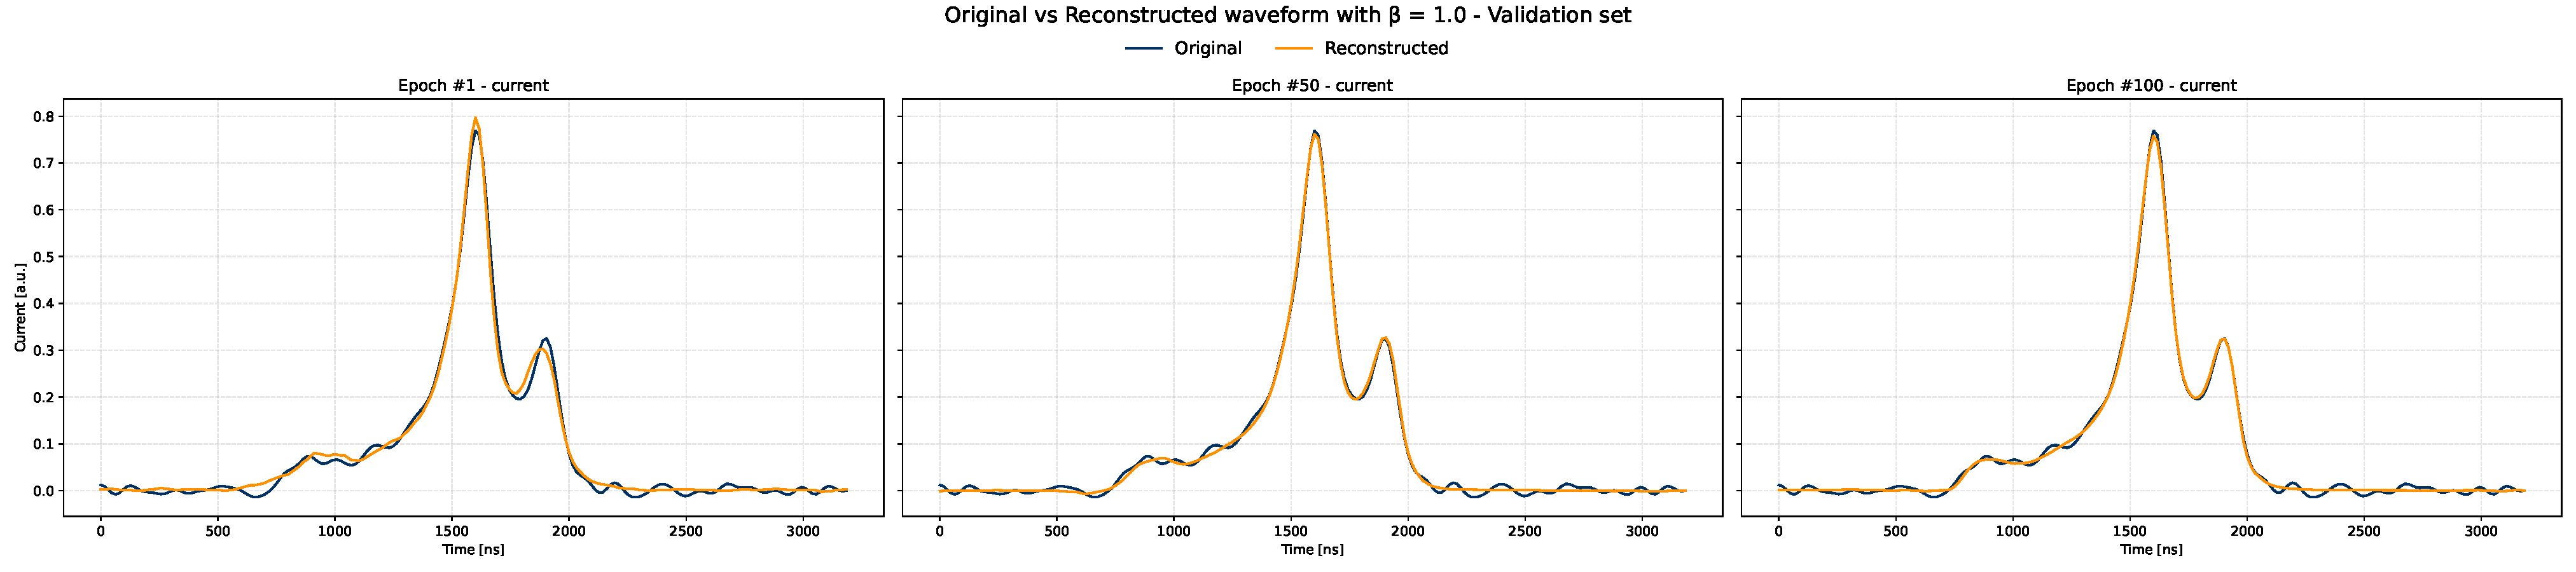
\includegraphics[width=\textwidth]{plots/VAEresults/beta1_sigma3_current_raw/validation_perEpoch_sigma3_current_raw_beta1.pdf}
    \caption{Decoder reconstrucion of validation set waveforms at epoch 1, 50 and 100}
    \label{fig:esempio-ricostruzione}
\end{figure}


\begin{figure}[H]
    \centering
    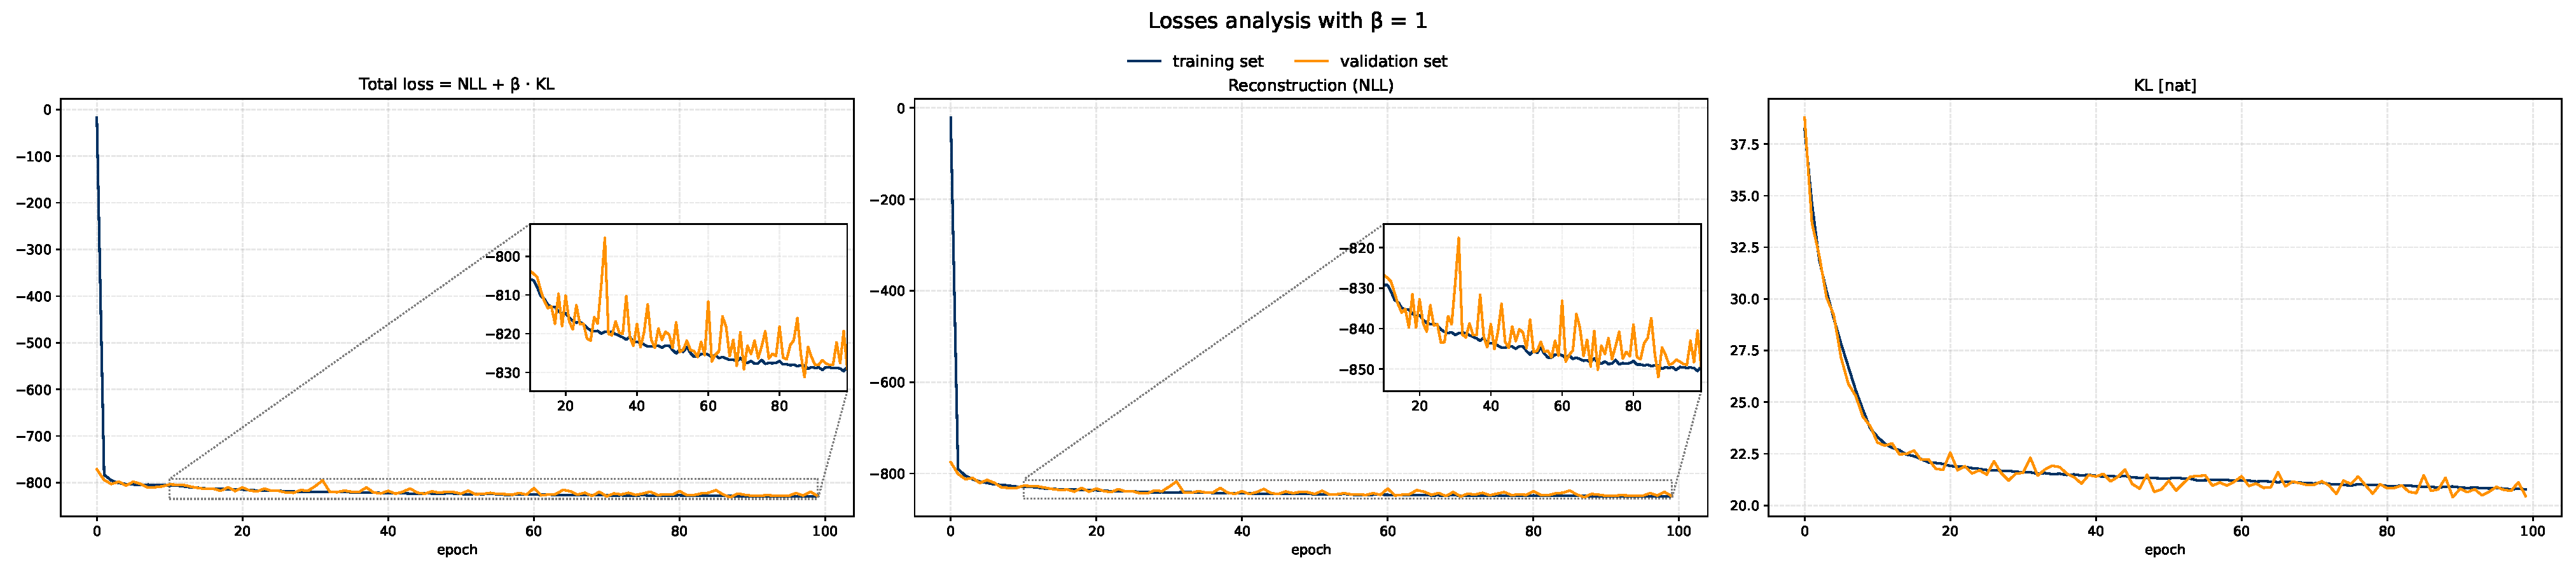
\includegraphics[width=\textwidth]{plots/VAEresults/beta1_sigma3_current_raw/train_valid_losses_sigma3_current_raw_beta1.pdf}
    \caption{Loss functions evolution through the training epochs. From the left to the right: total loss, reconstruction (\ac{NLL}) loss and \ac{KL} loss}
    \label{fig:esempio-losses}
\end{figure}



\subsection{\ac{VAE} as a feature extractor}
\label{subsec:VAE-features_extraction}
using beta1 and sigma3 

--- SSE SF with classifier = 59.95\% ---

--- MSE SF with classifier = 20.07\% ---

--- SSE SF with A/E = 59.10\% ---

--- MSE SF with A/E =  19.16\% ---

insomma uno schifo
\subsection{\ac{VAE} as a denoising algorithm}
\label{subsec:VAE-denoising}

\newpage
\section{Deep Temporal Clustering}
\label{sec:DTC}
As already mentioned, the main problem that affects the \ac{AE} method in the \ac{SSE}-\ac{MSE} discrimination is related to the fact that a complex waveform with its own evolution in time is treated and calssified on the basis of a single number. This number should in principle be a simple summary of the behaviour of the signal, but actually does not account for the time evolution of it. This problem is still present in a certain way also in the \ac{VAE}-based classifier: even though we use 8 features (and not only one), these are striclty correlated with single physical quantities that could ideally be computed by hand. Therefore what is really needed is a deep learning model that collapses all dimensions but the temporal one. On top of that, a features extraction aimed at a classification task separates the two goals of getting a good reconstruction of the waveform, which means having learnt important features of it, from the clustering problem.

Madiraju et al. (2018) in their paper \textit{"Deep Temporal Clustering: fully unsupervised learning of time-domain features"} \cite{DTC} implemented an algorithm, called Deep Temporal Clustering, aimed at unsupervised clustering of time series data. Firstly an autoencoder is used to extract a latent-space representation in time of the input data and secondly a clustering algorithm assigns said latent representation to a time series prototype, i.e. the equivalent of a centroid in K-Means algorithms. A number of prototypes, equals to the number of clusters we need to identify, is predefined and then tuned during the clustering training in order to resemble a typical waveform of a given cluster. The power of this network lays in two specific aspects: first the fact that the time dimension is preserved also in the latent representation and second the fact that exploiting a combined optimisation of the two branches of the complexive model, i.e. the autoencoding and the clustering, spatio-temporal features are extracted in order to optimise the reconstruction \textit{and} the clustering simoultaneously. 
\subsection{Architecure} 
The \ac{DTC} algorithm implemented for this work follows the one of the original paper\footnote{The full code of the authors is available here: \url{https://github.com/FlorentF9/DeepTemporalClustering}.}, but introduces several modifications and improvements, most notably the transition from the original Keras implementation to PyTorch. The overall architecure can be decomposed into two main parts: the autoencoder, specifically called \ac{TAE}, and the clustering referred to as \ac{TSC}. 

\subsubsection{Temporal Autoencoder class}
The \ac{TAE} is an Autoencoder for which the latent space is given by a compacted time series which ideally represents the input and from which the latter can be reconstructed with the decoder.
The workflow of the \ac{TAE} follows this scheme:
\begin{itemize}
    \item \textbf{input waveforms}\\
    Input waveforms are current signals processed as explained above in Sec. \ref{sec:data-cleaning} with dimension ($1~\times~200$). The only difference with respect to the \ac{VAE} input is that in this case no \ac{SSE}/\ac{MSE} cut has been performed and the whole energy spectrum between $1550$ keV and $1650$ keV has been considered. 
    \item \textbf{temporal encoder}\\
    The temporal encoder is constructed as a sequential module \cite{torchSequential}
    \begin{enumerate}
        \item a 1D convolutional (\texttt{Conv1d}) layer with kernel size = 10, stride = 1 and padding = kernel size - 1 = 10 - 1 = 9\footnote{This is the default configuration of padding when stride = 1. This padding value will be the same in all convolutional layers of this class.}, mapping the ($1~\times~200$) input into a tensor with dimensions ($50~\times~200$);
        \item a LeakyReLU activation function, already detailed in Eq. \ref{eq:leakyReLU}, with $\alpha = 0.1$;
        \item a 1D max pooling layer (\texttt{MaxPool1d}) with kernel size = 10 returnin a ($50~\times~20$) object and thus significantly reducing the time dimensions; this first two layers, i.e. the convolutional and the pooling layers, are needed in order to obtain a more compact representation of time series: dimensionality reduction is needed for the following steps to avoid very long sequences that may lead to a bad performance.
        \item a bidirectional \ac{LSTM} (\texttt{LSTM}) receiving the 50 input features that uses 50 hidden units to return another ($50\times~20$) object. Specifically a \ac{LSTM} is used to learn temporal changes in both time directions. Since the standard PyTorch library does not natively implement the summation of the forward and backward outputs, a dedicated custom class was designed to perform this operation manually;
        \item a LeakyReLU activation function with $\alpha = 0.1$;
        \item another bidirectional \ac{LSTM} with only one hidden unit to compact features in a single tensor of dimensions ($1~\times~20$);
        \item a LeakyReLU activation function with $\alpha = 0.1$.
    \end{enumerate}
    \item \textbf{latent space}\\
    Differently respect to the \ac{VAE} case, the latent space is a compact time series with dimensions ($1~\times~20$), i.e. the output of the last layer of the encoder module. This representation maintains the sequential nature of input data but extract significant features that are indeed the output of both the decoder module and the clustering layer that will be discussed further in this Section.
    \item \textbf{temporal decoder}\\
    The decoder part tries to reconstruct the original waveform, starting from the latent-space small time series. In \cite{DTC} the decoder constited of a upsampling layer followed by a deconvolutional one. After preliminary trials where a very bad reconstruction was observed the following architecture has been preferred:
    \begin{enumerate}
        \item a 1D convolutional layer: 50 kernels of kernel size = 10, stride = 1 and padding = kernel size $-1$ = 10 $-1$ = 9 expands the ($1 \times 20$) object up to a ($50 \times 20$) dimensionality object, without changing the temporal resolution;
        \item a LeakyReLU activation is performed on the output of the previous layer with $\alpha = 0.1$;
        \item the ($50 \times 20$) object is upsampled in linear mode, with a scaling factor that returns a ($50 \times 200$) object;
        \item a 1D convolutional layer with kernel size = 10, stride = 1 and padding = kernel size $-1$ = 10 $-1$ = 9 maps the 50 features back to the original number of channels, that is exactly 1, giving the final ($1 \times 200$) reconstructed waveform.
    \end{enumerate}
    \item \textbf{output waveforms}\\
    Just as in the \ac{VAE} implementation, output waveforms are the latent-based reconstruction of input ones.
\end{itemize}

Although the original loss function used in \cite{DTC} was a Mean Square Error loss, this is not suitable for our signals, as already discussed in \ref{subsec:VAE-training}. Thus loss function that parametrises and corrects all of the just-mentioned steps of the \ac{TAE} part of \ac{DTC} is a \ac{NLL} as the one of Eq. \ref{eq:rec-loss}. Therefore the \ac{TAE} loss function results in Eq. \ref{eq:tae-loss}, where $\sigma$ is a trainable parameter of the model here as well as in the \ac{VAE} implementation. Specifically, this parameter is tuned in the initial part of the training, called \textit{pretrain}, where only the \ac{TAE} is used, and then fixed for the second part of the training where also the \ac{TSC} part is implemented. 
% The architecture can also be visualised in Fig.~\ref{fig:tae-architecure}.

\begin{equation}
    \label{eq:tae-loss}
    L_{\text{TAE}} = \frac{1}{B} \sum_{i=1}^{B} \left[ \frac{1}{2} \sum_{t=1}^{T} \left( \frac{\left( x_{i,t} - \hat{x}_{i,t} \right)^2}{\sigma^2} + \log \sigma^2 \right) \right]
\end{equation}

\begin{figure}[H]
    \centering
    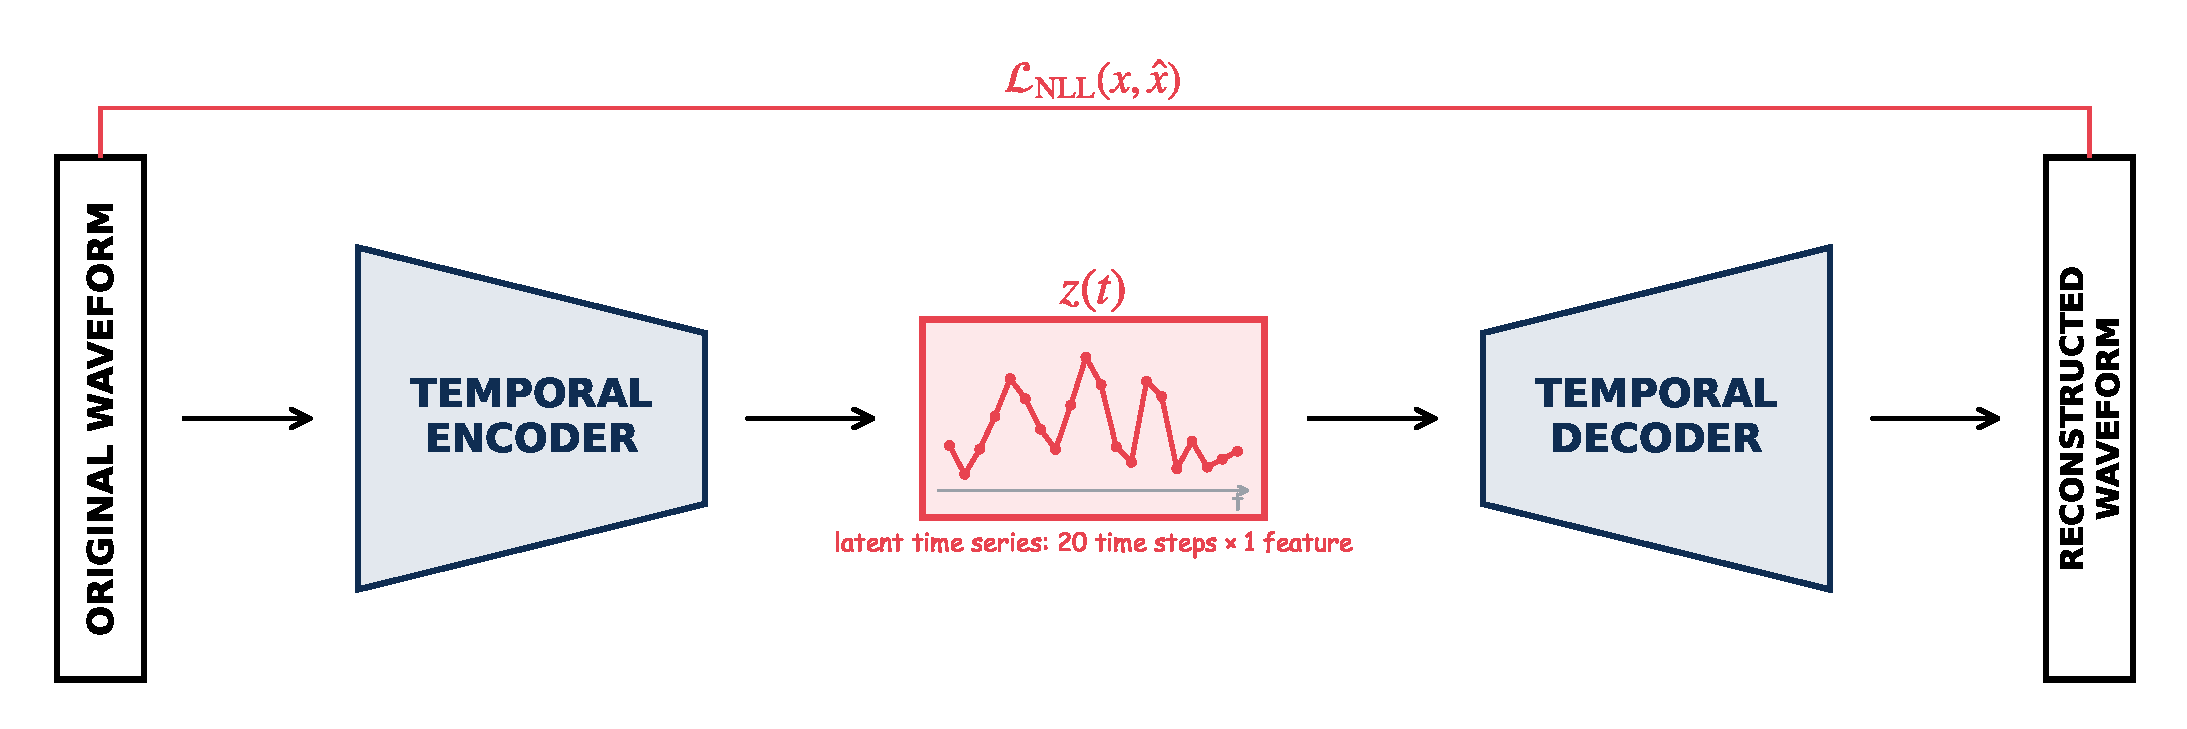
\includegraphics[width=\textwidth]{figures/schemi_output/TAE.pdf}
    \caption{Schematich representation of the \ac{TAE} architecture. The (temporal) endoer maps the input waveforms to a small time series in the latent space and the (temporal) decoder reconstruct waveforms from it. The model is mediated by a \ac{NLL} loss function.}
    \label{fig:tae-architecure}
\end{figure}

\subsubsection{Time Series Clustering class}
\label{subsubsec:TSC-class}
The \ac{TSC} class only consists of a tesorial object in the \texttt{Parameter} PyTorch class which represents the centroids for each class. Therefore this tensor parameter has dimensions (\texttt{clusters} $\times$ \texttt{length} $\times$ \texttt{features}) where the number of clusters is to be defined depending on how many different physical clusters we want to individuate and input length and channels are the ones of the latent representation of our input waveforms in the \ac{TAE}, in our case (\texttt{length} $\times$ \texttt{features}) = ($20~\times~1$). The cluster centroids tensor is first filled using the Xavier uniform initialisation \cite{Xavier}, which only acts as a placeholder: any non-constant initialisation breaks the symmetry between the centroids, whereas identical centroids would receive identical assignments ($q_{ij} = 1/k$) and zero gradients, and could never separate. Before the joint training, these values are overwritten by the centroids obtained by running KMeans on the latent representations of the training set, produced by the pre-trained \ac{TAE}\footnote{The original \ac{DTC} work uses hierarchical clustering with complete linkage for this step.}.
 The workflow of this class includes different steps:
\begin{itemize}
    \item \textbf{input acquisition}\\
    The clustering module receives the latent-space time sequences produced by the temporal encoder. Since standard 1D convolutional layers output tensors with dimensions ordered as (\texttt{features}~$\times$~\texttt{time steps}) = ($1~\times~20$), the latent tensor is first permuted to swap the channel and time axes. This yields a tensor with the expected shape of (\texttt{time steps}~$\times$~\texttt{features}) = ($20~\times~1$) in our setup. Finally, the permuted tensor is expanded along a new axis, preparing it for a broadcasted distance computation against all cluster centroids simultaneously, therefore obtaining ($1~\times~20\times~1$).
    \item \textbf{distance computation}\\
    A distance metric is computed between the input and each of the clusters centroids. Implemented metric distances are:
    \begin{itemize}
        \item \textbf{Euclidean Distance (EUC)}: given a latent sequence $x$ and a cluster centroid $w$, both made of $T$ time steps ($T = 20$, i.e. the input length divided by the pooling size), the distance is the usual geometrical distance of Eq. \ref{eq:EUC-distance}. Although it is the simplest and most intuitive metric, it compares the two sequences point by point, so it reacts to any difference in level, scale and timing between them. This is partly desirable, since the amplitude of the current carries the A/E information, but it also makes the metric sensitive to residual misalignments and noise, which can obscure the pulse-shape differences between SSE and MSE events\footnote{The alignment on the first current peak and the low-pass filter described in Sec. \ref{sec:data-cleaning} reduce these effects, but cannot remove them completely.}.
        \begin{equation}
            \label{eq:EUC-distance}
            d_\text{EUC}(x, w) = \sqrt{\sum_{t=1}^{T} (x_{t} - w_{t})^2}
        \end{equation}

        \item \textbf{Complexity-Invariant Distance (CID)}: this metric, introduced by Batista et al. \cite{Batista}, extends the Euclidean distance with a correction factor based on the complexity of the time series, which prevents two sequences with very different variability from being considered close. The complexity estimate $\mathrm{CE}$ of a series (Eq. \ref{eq:CE-factor}) is the norm of its discrete derivative, i.e. the square root of the sum of the squared differences between consecutive points. The final distance is the Euclidean distance multiplied by the ratio between the larger and the smaller complexity (Eq. \ref{eq:CID-distance}); this factor is always $\geq 1$ and equals 1 only when the two sequences have the same complexity.
        \begin{equation}
            \label{eq:CE-factor}
            \mathrm{CE}(x) = \sqrt{\sum_{t=1}^{T-1} (x_{t+1} - x_t)^2}
        \end{equation}
        \begin{equation}
            \label{eq:CID-distance}
            d_\text{CID}(x, w) = d_\text{EUC}(x, w) \cdot \frac{\max[\mathrm{CE}(x), \mathrm{CE}(w)]}{\min[\mathrm{CE}(x), \mathrm{CE}(w)]}
        \end{equation}

        \item \textbf{Auto-Correlation Function (ACF)}: this metric was introduced by Galeano \& Pe\~{n}a \cite{Galeano} and compares the latent sequence and the centroid through a weighted Euclidean distance between their autocorrelation coefficients. First, both sequences are converted into their sample autocorrelation functions $\varrho_x$ and $\varrho_w$ (Eq. \ref{eq:ACF}), computed for all the lags $k = 0, \dots, T-1$:
        \begin{equation}
            \label{eq:ACF}
            \varrho_x(k) = \frac{\sum_{t=1}^{T-k} (x_t - \bar{x})(x_{t+k} - \bar{x})}{\sum_{t=1}^{T} (x_t - \bar{x})^2}
        \end{equation}
        where $\bar{x}$ is the mean of the sequence. Since the mean is subtracted and the result is divided by the variance, $\varrho_x$ is invariant under any rescaling and shift of the latent sequence: it keeps only its temporal correlation structure, i.e. the width of the peaks and the separation between them, which shows up as a secondary bump of $\varrho_x$ at the corresponding lag. Second, a decaying diagonal matrix $\boldsymbol{\Omega}$ (Eq. \ref{eq:Omega-matrix}, with $m = T$) gives more weight to the lower lags: the coefficient at lag $k$ is estimated from only $T-k$ pairs of points, so the coefficients at high lags are the least reliable and are progressively suppressed.
        \begin{equation}
            \label{eq:Omega-matrix}
            \begin{aligned}
                \boldsymbol{\Omega} &= \begin{bmatrix} 
                \omega_0 & 0 & \cdots & 0 \\ 
                0 & \omega_1 & \cdots & 0 \\ 
                \vdots & \vdots & \ddots & \vdots \\ 
                0 & 0 & \cdots & \omega_{m-1} 
                \end{bmatrix} \\[1ex]
                \omega_k &= 1 - \frac{k}{m-1} \quad \text{for } k = 0, 1, \dots, m-1
            \end{aligned}
        \end{equation}
        Finally, the differences between the two autocorrelation functions are quantified as in Eq. \ref{eq:AC-distance}. Note that $\varrho(0) = 1$ for every sequence and $\omega_{m-1} = 0$, so neither the first nor the last lag contributes to the distance.
        \begin{equation}
            \label{eq:AC-distance}
            d_{\text{ACF}}(x, w) = \sqrt{(\varrho_x - \varrho_w)^{\top} \boldsymbol{\Omega} \, (\varrho_x - \varrho_w)}
        \end{equation}
    \end{itemize}
    \item \textbf{probability calculation}:\\
    The probability of belonging to a given cluster $j$ is based on a t-Student distribution kernel. Specifically, the similarity between the latent representation of a sample $x_i$ and a cluster centroid $w_j$ is evaluated using a Student's t-distribution with $\alpha$ degrees of freedom as a kernel. While the theoretical probability density function of the t-distribution includes a normalization constant defined by the Gamma function $\Gamma(\cdot)$, this term cancels out during the cluster assignment phase. In fact, to obtain valid soft assignments (i.e., probabilities that sum to 1), the score of cluster $j$ is normalized by the sum of the scores over all $k$ clusters \cite{DTC}. Since the degrees of freedom parameter $\alpha$ is a global constant across all clusters, the $\Gamma$ term simplifies algebraically, yielding the final probability $q_{ij}$ defined in Eq. \ref{eq:q-prob}:
    \begin{equation}
        \label{eq:q-prob}
        q_{ij} = \frac{\left( 1 + \frac{d(x_i, w_j)^2}{\alpha} \right)^{-\frac{\alpha+1}{2}}}{\sum_{k=1}^{K} \left( 1 + \frac{d(x_i, w_k)^2}{\alpha} \right)^{-\frac{\alpha+1}{2}}}
    \end{equation}
    where $d(x_i, w_j)$ is the distance metric chosen among the ones previously described, and $\alpha$ controls the heaviness of the distribution tails. From an architectural perspective, the heavy tails of the t-Student distribution are preferred over a standard Gaussian kernel because they prevent vanishing gradients for samples located far from the centroids, resulting in a more robust training process.
    \item \textbf{target distribution definition}:\\
    Being the \ac{DTC} a fully unsupervised method, a self-training mechanism is employed: seeing that the model doesn't have any target label, a target distribution built from $q_{ij}$ probabilities themselves is constructed, following the one in \cite{DTC}.
    Eq. \ref{eq:target-distribution-p} mathematically explains how said distribution is defined: Squaring $q_{ij}$ amplifies the most confident predictions, while $f_j$ (Eq.~\ref{eq:frequency-j}) is the soft frequency of cluster $j$, i.e. the sum of the assignment probabilities over the $B$ samples of the batch\footnote{In \cite{DTC} $f_j$ is computed over the whole dataset.}, so that dividing by it penalises very large clusters. The ratio $q^{2}_{ij}/f_j$ is then normalised over all the $K$ clusters.
    \begin{equation}
        \label{eq:target-distribution-p}
        p_{ij} = \frac{q^{2}_{ij} / f_j}{\sum_{k=1}^{K} q^{2}_{ik} / f_k}
    \end{equation}
    \begin{equation}
        \label{eq:frequency-j}
        f_j = \sum_{i=1}^{B} q_{ij}
    \end{equation}
\end{itemize}



Finally, the loss is computed as a \ac{KL} divergence, similar to the one used in Sec.~\ref{sec:vae-architeture}, averaged over the $B$ samples of a batch:

\begin{equation}
    \label{eq:KL-loss-TSC}
    L_{KL} = \frac{1}{B} \sum_{i=1}^{B} \sum_{j=1}^{K} p_{ij} \log \frac{p_{ij}}{q_{ij}}
\end{equation}

The target distribution is computed from the current $q_{ij}$ but it is treated as a constant, so that no gradient flows through it. Minimising Eq.~\ref{eq:KL-loss-TSC} therefore pushes $q_{ij}$ towards a sharper version of itself. Since $p_{ij}$ is recomputed at every update, the two distributions never simply coincide: as the assignments become more confident, so does the target, and the training converges towards high-confidence assignments.

Being \texttt{Parameter} objects, the centroids $w_j$ are optimised together with the weights of the \ac{TAE}, starting from the K-Means initialisation, by gradient descent on the total loss $L = L_\text{TAE} + \gamma \cdot L_{KL}$. However, seeing that $L_\text{TAE}$ does not depend on the centroids, they are moved only by the clustering term. For the Euclidean distance, $d_{ij}^2 = \lVert z_i - w_j \rVert^2$, the gradients are~\cite{KL-backpropagation}:

\begin{align}
    \frac{\partial L_{KL}}{\partial w_j} &= -\frac{\alpha+1}{\alpha B} \sum_{i=1}^{B} \left(1 + \frac{d_{ij}^2}{\alpha}\right)^{-1} (p_{ij} - q_{ij})\,(z_i - w_j) \label{eq:grad-centroids} \\
    \frac{\partial L_{KL}}{\partial z_i} &= \frac{\alpha+1}{\alpha B} \sum_{j=1}^{K} \left(1 + \frac{d_{ij}^2}{\alpha}\right)^{-1} (p_{ij} - q_{ij})\,(z_i - w_j) \label{eq:grad-latent}
\end{align}

Eq.~\ref{eq:grad-centroids} has an intuitive interpretation: if the target assigns sample $i$ to cluster $j$ with more confidence than the model ($p_{ij} > q_{ij}$), the gradient step moves the centroid $w_j$ towards $z_i$, while if $p_{ij} < q_{ij}$ it moves it away. The factor $(1 + d_{ij}^2/\alpha)^{-1}$ gives more weight to the samples that are already close to the centroid. At the same time, Eq.~\ref{eq:grad-latent} is back-propagated through the encoder, so that the latent representation $z_i$ of each sample is pulled towards the centroid of the cluster it most likely belongs to: the clustering reshapes the latent space itself, while $L_{NLL}$ keeps it faithful to the input waveforms. For the Complexity-Invarian Distance and the Autocorrelation Function the gradients follow from the same chain rule and are computed by automatic differentiation.


The full \ac{DTC} model that includes both the \ac{TAE} and the \ac{TSC} is shown in Fig.~\ref{fig:tae_and_tsc-architecure}.
\begin{figure}[H]
    \centering
    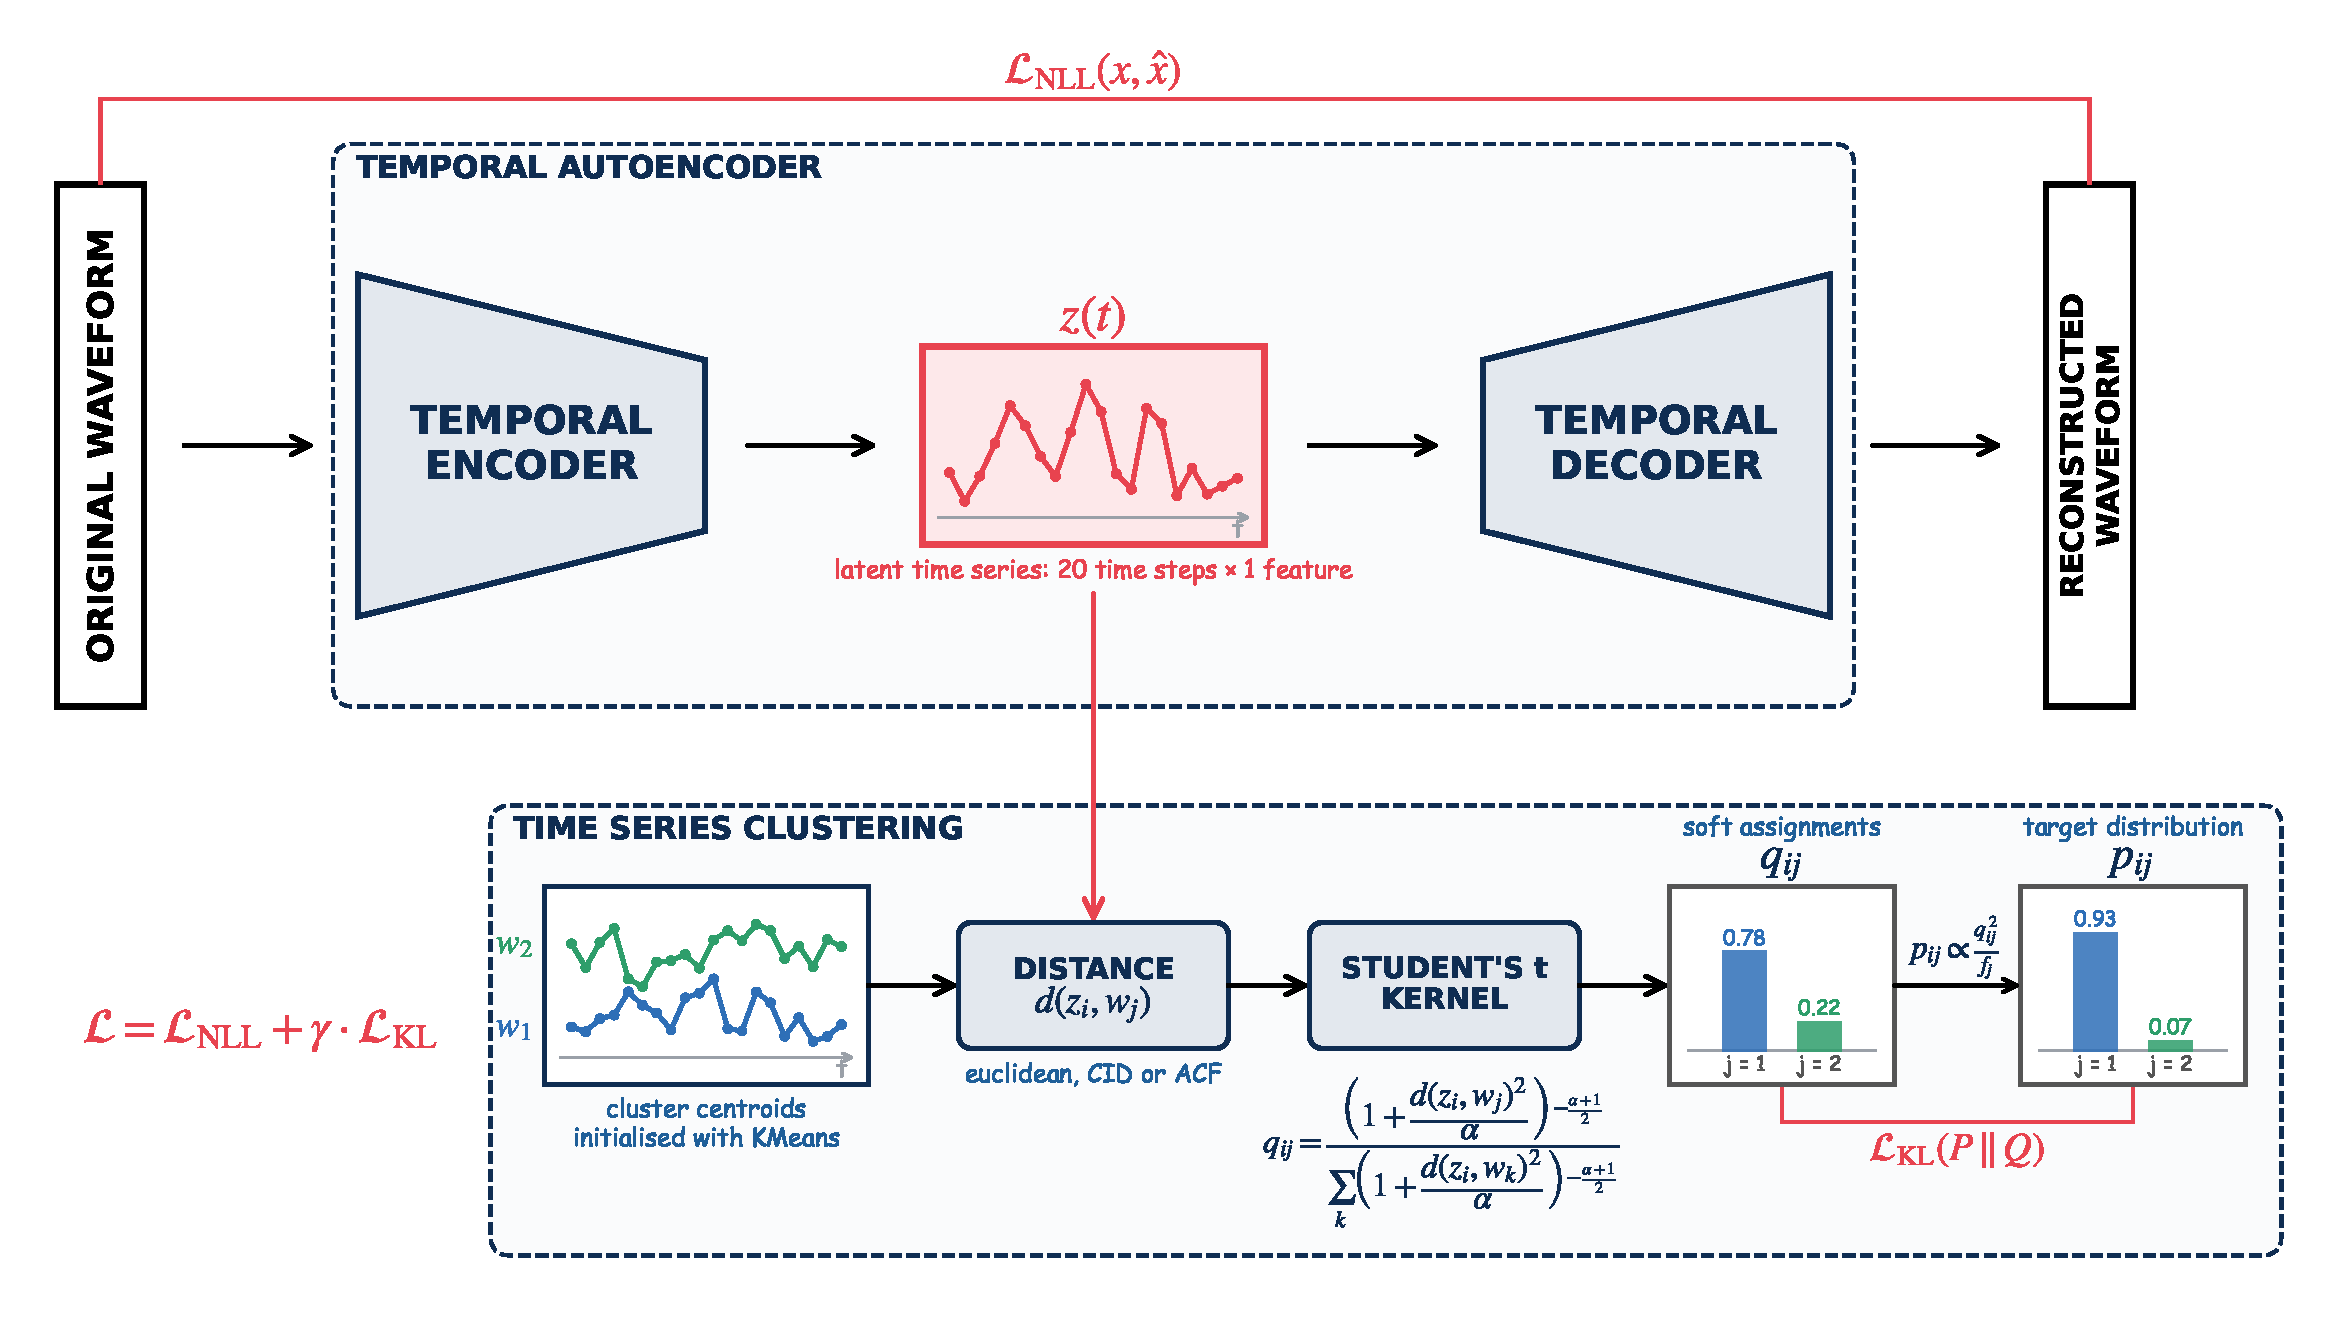
\includegraphics[width=\textwidth]{figures/schemi_output/TAE_clustering.pdf}
    \caption{Schematich representation of the \ac{DTC} architecture. The (temporal) encoder maps the input waveforms to a small time series in the latent space and the (temporal) decoder reconstruct waveforms from it. Moreover the time-series latent space is used to separate waveforms in different clusters. The full model is mediated by the \ac{NLL} loss function for the \ac{TAE} and the \ac{KL} divergence for the \ac{TSC}.}
    \label{fig:tae_and_tsc-architecure}
\end{figure}


\subsection{Data selection}
Being a fully-unsupervised clustering algorithm, the \ac{DTC} model does not require a specific data selection before its training. Therefore all the events in the 1550-1650 keV range of the calibration dataset, i.e. the whole gray spectrum of Fig.~\ref{fig:distribution-AoE_prl25}, have been employed as input waveforms of this algorithm, for a total $N_\text{DTC} = 348 999$ waveforms divided in the training, validation and test set as detailed in Table \ref{tab:sets-DTC}.
\begin{table}[H]
    \centering
    \begin{tabular}{cc}
        \toprule
        set & number of waveforms\\
        \midrule
        training & 279 199 \\
        validation & 34 900 \\
        test & 34 900\\
        \bottomrule
    \end{tabular}
    \caption{Division of events between the training, validation and test sets for the \ac{DTC} model.}
    \label{tab:sets-DTC}
\end{table}

The validation set has been used in this model, as well as in the previous one, to make sure the model does not overfit and to monitor that both the training and validation loss are decreasing through epochs.


\subsection{Training and testing}
The \ac{DTC} training phase is divided in two different parts: the \textit{pretrain}, where only the \ac{TAE} is used and then the proper \textit{train} where both the \ac{TAE} and the \ac{TSC} are implemented. 

\textbf{\textit{Pretrain}}: this phase is used in order to make the model learning how to reconstruct the input waveforms from the latent representation, without being affected by the clustering algorithm. The loss function used is the one described in Eq. \ref{eq:tae-loss} and as already introduced the parameter $\sigma$ in this phase is a learnable parameter on which the backpropagation acts. The model is trained for a number of epochs $\text{N}_\text{PRE} = 40$. The reconstruction ability of the \ac{TAE} is shown in Fig. \ref{fig:pretrain-validation} for a waveform in the validation set at different epochs. Fig. \ref{fig:pretrain-loss} shows the \ac{NLL} loss evolution: it is evident that both the training set loss and the validation one decreases over time, ensuring the fact that the model is actually learning how to recontruct waveforms and it is not overfitting training data.
\begin{figure}[H]
    \centering
    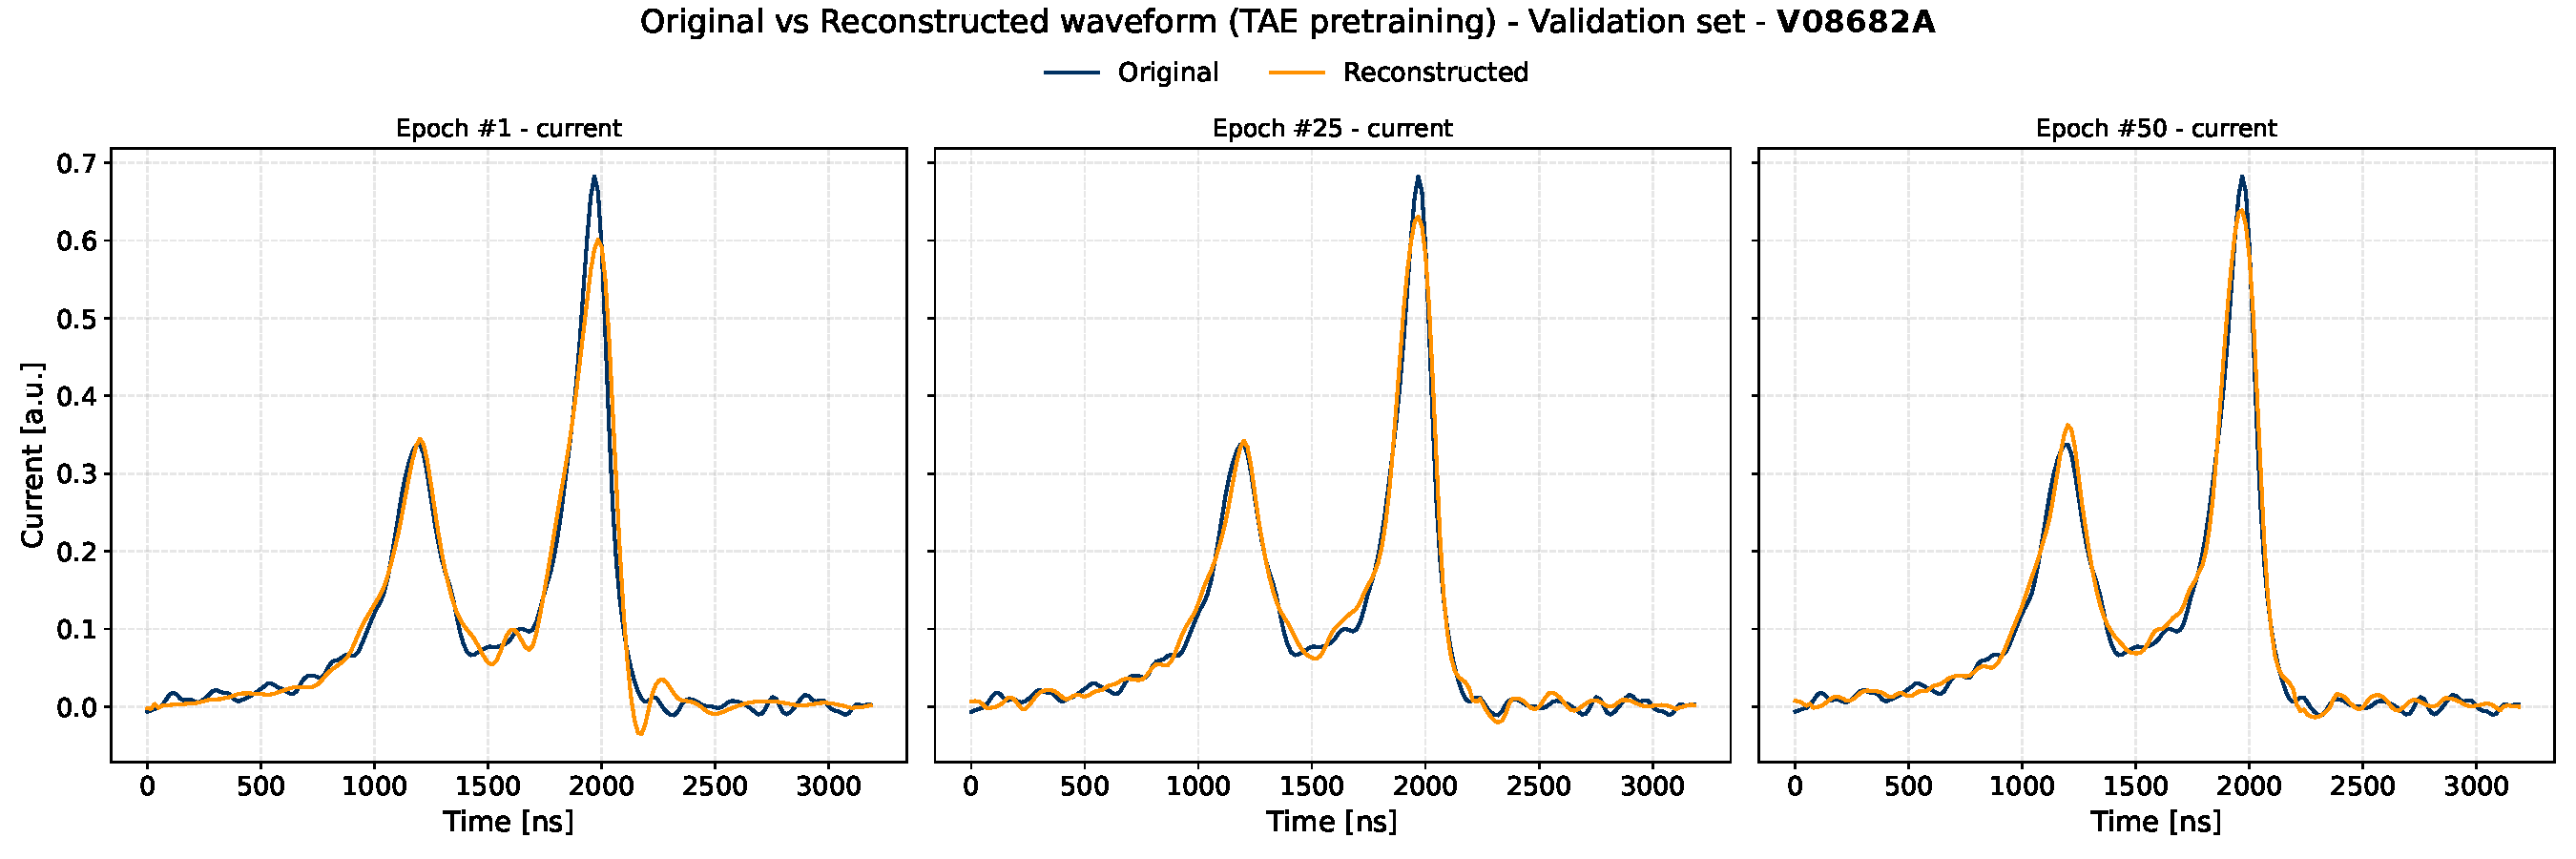
\includegraphics[width=\textwidth]{plots/DTC/pretrain_reconstruction.pdf}
    \caption{Example of the \ac{TAE} reconstruction ability in the \textit{pretrain} for a validation set waveform at epoch 1, 20, 40.}
    \label{fig:pretrain-validation}
\end{figure}

\begin{figure}[H]
    \centering
    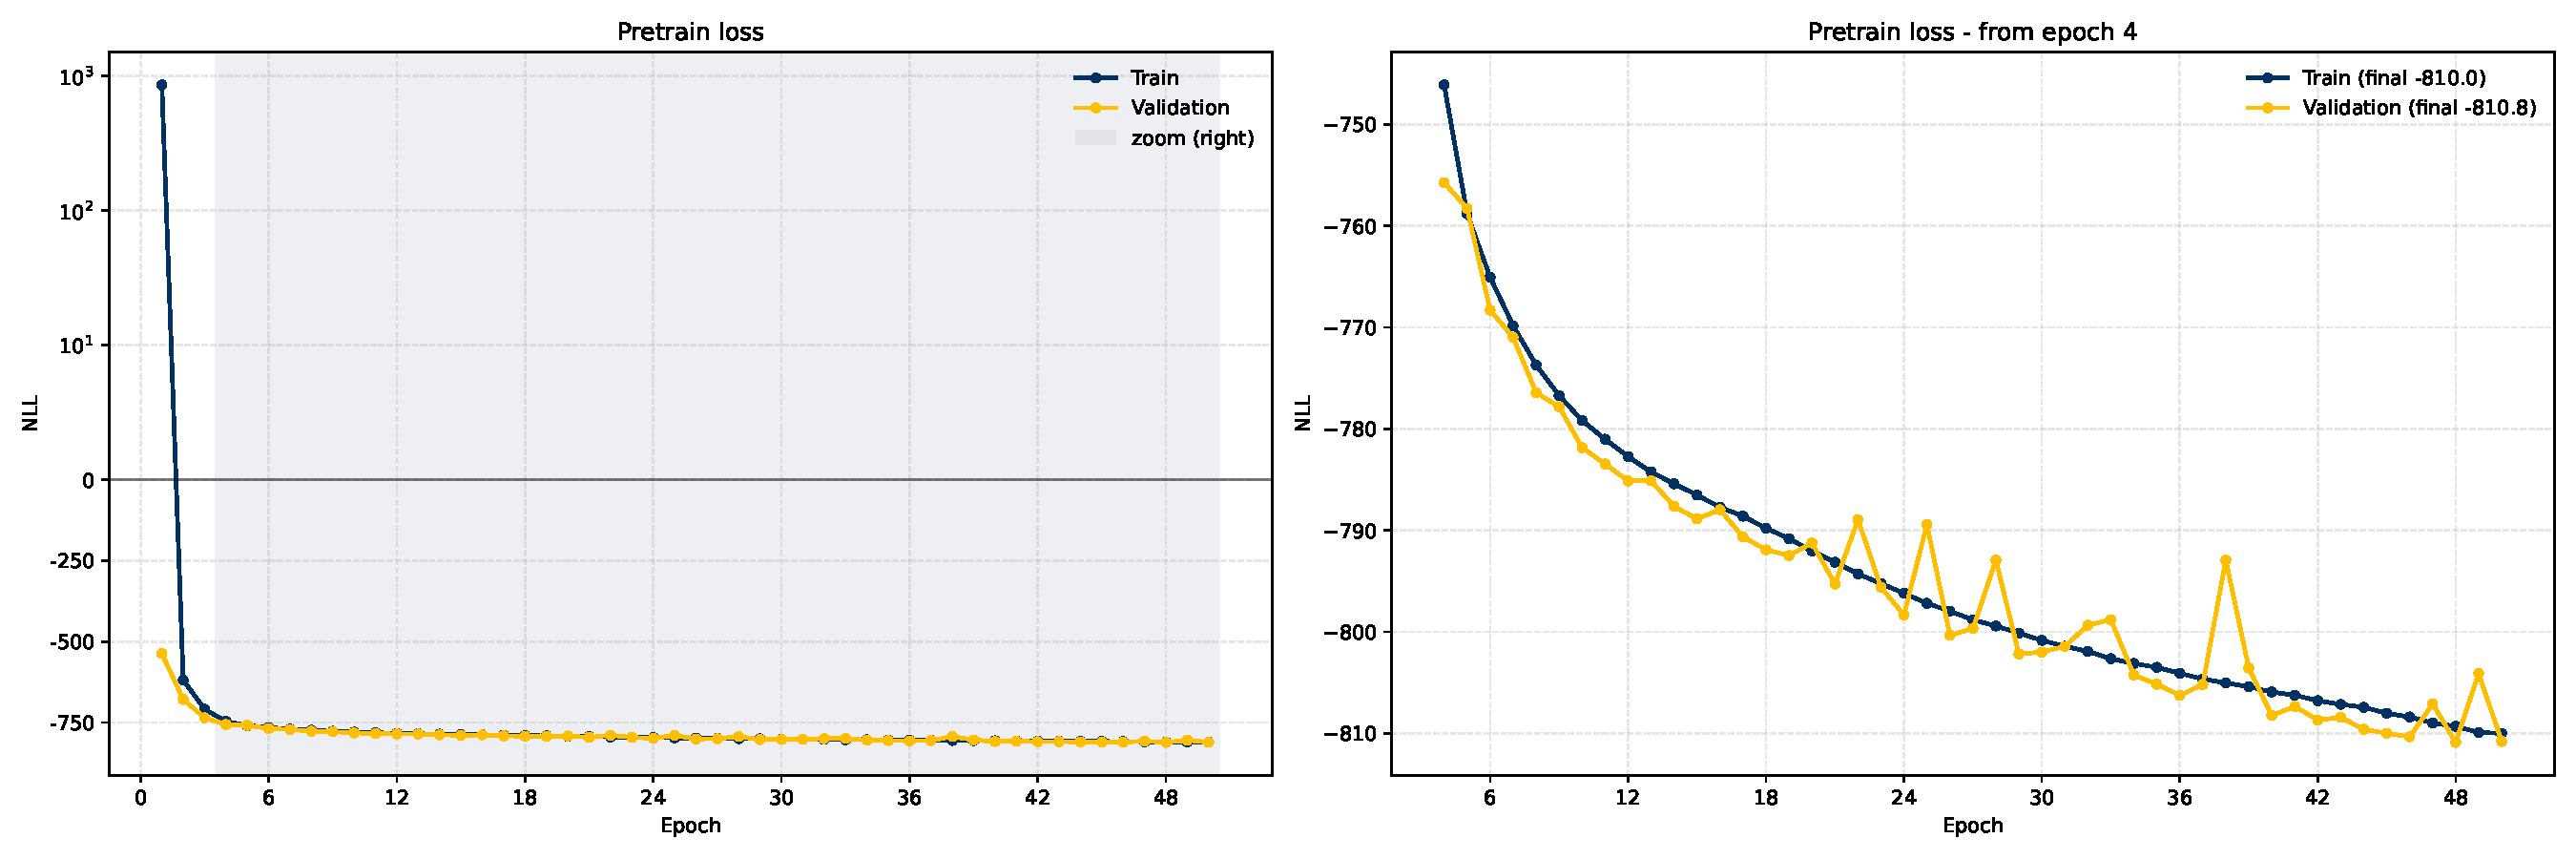
\includegraphics[width=\textwidth]{plots/DTC/pretrain_losses.pdf}
    \caption{\textit{Pretrain} loss evolution through epochs. On the right a zoom of the grey part of the left plot is shown.}
    \label{fig:pretrain-loss}
\end{figure}

Soon after this part is completed, the $\sigma$ parameter is fixed to the learned value and the centroids of the clusters are pre-initialised using a K-Means algorithm on the latent representation of the training set. It is from said centroids that the \ac{TSC} part of the mdoel starts to cluster waveforms.

\textbf{\textit{Train}}: in the second phase of the \ac{DTC} training, the proper \textit{training} phase, both the \ac{TAE} and the \ac{TSC} are used. As a consequence, the complexive loss function includes $L_\text{TAE}$ and $L_\text{TSC}$, weighted by a specific tunable parameter $\gamma$ in order to have the total loss of Eq. \ref{eq:total_dtc_loss}. Therefore the backpropagation acts both on the reconstruction of input waveforms and on the clustering of them simultaneously.
\begin{equation}
    \label{eq:total_dtc_loss}
    L_\text{DTC} = L_\text{TAE} + \gamma \cdot L_\text{TSC}
\end{equation}

The results of the complexive training part with $\text{N}_\text{TRAIN} = 20$ epochs and $\gamma = 1000$ are shown in Fig. \ref{fig:training-reconstruction-DTC}and \ref{fig:training-clustering-DTC} for the reconstruction and clustering part respectively and for all of the abovementioned distance metrics.
\begin{figure}[H]
    \centering
    
\includegraphics[width=0.5\textwidth]{plots/placeholder.png}
    \caption{\colorbox{yellow}{PLACEHOLDER}}
    \label{fig:training-reconstruction-DTC}
\end{figure}

\begin{figure}[H]
    \centering
    
\includegraphics[width=0.5\textwidth]{plots/placeholder.png}
    \caption{\colorbox{yellow}{PLACEHOLDER}}
    \label{fig:training-clustering-DTC}
\end{figure}




\newpage
\section{Self-Organising Map}
\label{sec:SOM}
A \ac{SOM} is an unsupervised machine learning tecnique used to produce low-dimensionality representation of a higher-dimensionality dataset preserving topological structures of data that distinguish different types of said data. Specifically, a \ac{SOM} is a type of artificial neural network trained using competitive learning rather than error-correction learning. The goal in these auto-organised learning maps is to train different parts of the \ac{SOM} to reply to different input patterns: this specific design has been formulated in the 1980s by Teuvo Kohonen on the basis of how the human brain manages different information in different parts of the cerebral cortex.

Starting from weights vectors initialised to casual or very small numbers, the algorithm exploits competitive learning: when a new training sample is received by the network, a distance metric is computed from all the weights vectors. The most alike weights vector, named \ac{BMU} and all the neurons near to ir in the \ac{SOM} net are brought closer with one another and weights are updated.